% !TEX program = XeLaTeX
%DIF LATEXDIFF DIFFERENCE FILE
%DIF DEL IPM - Nomura - before second review.tex   Wed Aug  1 01:47:05 2018
%DIF ADD IPM - Nomura.tex                          Wed Dec  5 18:05:38 2018
\documentclass[review]{elsarticle}

\usepackage{lineno,hyperref}
%DIF 5c5-6
%DIF < \usepackage{array, pbox}
%DIF -------
\usepackage{array} %DIF > 
\usepackage{appendix} %DIF > 
%DIF -------
\usepackage{mathtools}
% \usepackage{colortbl}
\usepackage[table]{xcolor}
\usepackage{caption}
%DIF 10a11-16
\usepackage{multirow} %DIF > 
\usepackage{lscape} %DIF > 
\usepackage{graphicx} %DIF > 
\usepackage{ntheorem} %DIF > 
\theoremseparator{:} %DIF > 
\newtheorem{hyp}{Hypothesis} %DIF > 
%DIF -------

\definecolor{DeepRed}{HTML}{990000}
\definecolor{DarkSalmon}{HTML}{ea9999}
\definecolor{Salmon}{HTML}{f4cccc}

\definecolor{DeepPurple}{HTML}{674ea7}
\definecolor{DarkLiliac}{HTML}{b4a7d6}
\definecolor{Liliac}{HTML}{d9d2e9}

\definecolor{DeepGreen}{HTML}{6aa84f}
\definecolor{DarkLime}{HTML}{b6d7a8}
\definecolor{LightGreen}{HTML}{d9ead3}

\definecolor{DarkBlue}{HTML}{6d9eeb}
\definecolor{LightBlue}{HTML}{c9daf8}

\definecolor{Plum}{HTML}{a64d79}
\definecolor{LightPlum}{HTML}{c27ba0}
%DIF 28a35
\definecolor{SweetPlum}{HTML}{dbaac4} %DIF > 
%DIF -------
\definecolor{Mustard}{HTML}{ffd966}
\definecolor{DeepSalmon}{HTML}{e06666}

\makeatletter
\newcommand*{\@rowstyle}{}
\newcommand*{\rowstyle}[1]{% sets the style of the next row
  \gdef\@rowstyle{#1}%
  \@rowstyle\ignorespaces%
}
\newcolumntype{=}{% resets the row style
  >{\gdef\@rowstyle{}}%
}
\newcolumntype{+}{% adds the current row style to the next column
  >{\@rowstyle}%
}
\makeatother

\modulolinenumbers[5]
\journal{Journal of Information Processing and Management}

%%%%%%%%%%%%%%%%%%%%%%%
%% Elsevier bibliography styles
%%%%%%%%%%%%%%%%%%%%%%%
%% To change the style, put a % in front of the second line of the current style and
%% remove the % from the second line of the style you would like to use.
%%%%%%%%%%%%%%%%%%%%%%%

%% Numbered
%\bibliographystyle{model1-num-names}

%% Numbered without titles
%\bibliographystyle{model1a-num-names}

%% Harvard
%\bibliographystyle{model2-names.bst}\biboptions{authoryear}

%% Vancouver numbered
%\usepackage{numcompress}\bibliographystyle{model3-num-names}

%% Vancouver name/year
%\usepackage{numcompress}\bibliographystyle{model4-names}\biboptions{authoryear}

%% APA style
%\bibliographystyle{model5-names}\biboptions{authoryear}

%% AMA style
%\usepackage{numcompress}\bibliographystyle{model6-num-names}

%% `Elsevier LaTeX' style
\bibliographystyle{elsarticle-num}
%%%%%%%%%%%%%%%%%%%%%%%
%DIF PREAMBLE EXTENSION ADDED BY LATEXDIFF
%DIF UNDERLINE PREAMBLE %DIF PREAMBLE
\RequirePackage[normalem]{ulem} %DIF PREAMBLE
\RequirePackage{color}\definecolor{RED}{rgb}{1,0,0}\definecolor{BLUE}{rgb}{0,0,1} %DIF PREAMBLE
\providecommand{\DIFaddtex}[1]{{\protect\color{blue}\uwave{#1}}} %DIF PREAMBLE
\providecommand{\DIFdeltex}[1]{{\protect\color{red}\sout{#1}}}                      %DIF PREAMBLE
%DIF SAFE PREAMBLE %DIF PREAMBLE
\providecommand{\DIFaddbegin}{} %DIF PREAMBLE
\providecommand{\DIFaddend}{} %DIF PREAMBLE
\providecommand{\DIFdelbegin}{} %DIF PREAMBLE
\providecommand{\DIFdelend}{} %DIF PREAMBLE
%DIF FLOATSAFE PREAMBLE %DIF PREAMBLE
\providecommand{\DIFaddFL}[1]{\DIFadd{#1}} %DIF PREAMBLE
\providecommand{\DIFdelFL}[1]{\DIFdel{#1}} %DIF PREAMBLE
\providecommand{\DIFaddbeginFL}{} %DIF PREAMBLE
\providecommand{\DIFaddendFL}{} %DIF PREAMBLE
\providecommand{\DIFdelbeginFL}{} %DIF PREAMBLE
\providecommand{\DIFdelendFL}{} %DIF PREAMBLE
%DIF HYPERREF PREAMBLE %DIF PREAMBLE
\providecommand{\DIFadd}[1]{\texorpdfstring{\DIFaddtex{#1}}{#1}} %DIF PREAMBLE
\providecommand{\DIFdel}[1]{\texorpdfstring{\DIFdeltex{#1}}{}} %DIF PREAMBLE
\newcommand{\DIFscaledelfig}{0.5}
%DIF HIGHLIGHTGRAPHICS PREAMBLE %DIF PREAMBLE
\RequirePackage{settobox} %DIF PREAMBLE
\RequirePackage{letltxmacro} %DIF PREAMBLE
\newsavebox{\DIFdelgraphicsbox} %DIF PREAMBLE
\newlength{\DIFdelgraphicswidth} %DIF PREAMBLE
\newlength{\DIFdelgraphicsheight} %DIF PREAMBLE
% store original definition of \includegraphics %DIF PREAMBLE
\LetLtxMacro{\DIFOincludegraphics}{\includegraphics} %DIF PREAMBLE
\newcommand{\DIFaddincludegraphics}[2][]{{\color{blue}\fbox{\DIFOincludegraphics[#1]{#2}}}} %DIF PREAMBLE
\newcommand{\DIFdelincludegraphics}[2][]{% %DIF PREAMBLE
\sbox{\DIFdelgraphicsbox}{\DIFOincludegraphics[#1]{#2}}% %DIF PREAMBLE
\settoboxwidth{\DIFdelgraphicswidth}{\DIFdelgraphicsbox} %DIF PREAMBLE
\settoboxtotalheight{\DIFdelgraphicsheight}{\DIFdelgraphicsbox} %DIF PREAMBLE
\scalebox{\DIFscaledelfig}{% %DIF PREAMBLE
\parbox[b]{\DIFdelgraphicswidth}{\usebox{\DIFdelgraphicsbox}\\[-\baselineskip] \rule{\DIFdelgraphicswidth}{0em}}\llap{\resizebox{\DIFdelgraphicswidth}{\DIFdelgraphicsheight}{% %DIF PREAMBLE
\setlength{\unitlength}{\DIFdelgraphicswidth}% %DIF PREAMBLE
\begin{picture}(1,1)% %DIF PREAMBLE
\thicklines\linethickness{2pt} %DIF PREAMBLE
{\color[rgb]{1,0,0}\put(0,0){\framebox(1,1){}}}% %DIF PREAMBLE
{\color[rgb]{1,0,0}\put(0,0){\line( 1,1){1}}}% %DIF PREAMBLE
{\color[rgb]{1,0,0}\put(0,1){\line(1,-1){1}}}% %DIF PREAMBLE
\end{picture}% %DIF PREAMBLE
}\hspace*{3pt}}} %DIF PREAMBLE
} %DIF PREAMBLE
\LetLtxMacro{\DIFOaddbegin}{\DIFaddbegin} %DIF PREAMBLE
\LetLtxMacro{\DIFOaddend}{\DIFaddend} %DIF PREAMBLE
\LetLtxMacro{\DIFOdelbegin}{\DIFdelbegin} %DIF PREAMBLE
\LetLtxMacro{\DIFOdelend}{\DIFdelend} %DIF PREAMBLE
\DeclareRobustCommand{\DIFaddbegin}{\DIFOaddbegin \let\includegraphics\DIFaddincludegraphics} %DIF PREAMBLE
\DeclareRobustCommand{\DIFaddend}{\DIFOaddend \let\includegraphics\DIFOincludegraphics} %DIF PREAMBLE
\DeclareRobustCommand{\DIFdelbegin}{\DIFOdelbegin \let\includegraphics\DIFdelincludegraphics} %DIF PREAMBLE
\DeclareRobustCommand{\DIFdelend}{\DIFOaddend \let\includegraphics\DIFOincludegraphics} %DIF PREAMBLE
\LetLtxMacro{\DIFOaddbeginFL}{\DIFaddbeginFL} %DIF PREAMBLE
\LetLtxMacro{\DIFOaddendFL}{\DIFaddendFL} %DIF PREAMBLE
\LetLtxMacro{\DIFOdelbeginFL}{\DIFdelbeginFL} %DIF PREAMBLE
\LetLtxMacro{\DIFOdelendFL}{\DIFdelendFL} %DIF PREAMBLE
\DeclareRobustCommand{\DIFaddbeginFL}{\DIFOaddbeginFL \let\includegraphics\DIFaddincludegraphics} %DIF PREAMBLE
\DeclareRobustCommand{\DIFaddendFL}{\DIFOaddendFL \let\includegraphics\DIFOincludegraphics} %DIF PREAMBLE
\DeclareRobustCommand{\DIFdelbeginFL}{\DIFOdelbeginFL \let\includegraphics\DIFdelincludegraphics} %DIF PREAMBLE
\DeclareRobustCommand{\DIFdelendFL}{\DIFOaddendFL \let\includegraphics\DIFOincludegraphics} %DIF PREAMBLE
%DIF END PREAMBLE EXTENSION ADDED BY LATEXDIFF

\begin{document}

\begin{frontmatter}

\title{Measuring the Influence of Mere Exposure Effect of TV Commercial Adverts on Purchase Behavior based on Machine Learning Prediction Models}

\author[gidai]{Elisa Claire Alemán Carreón
\corref{mycorrespondingauthor}}
\ead{s153400@stn.nagaokaut.ac.jp}

\author[gidai]{Hirofumi Nonaka}
\ead{nonaka@kjs.nagaokaut.ac.jp}

\author[gidai]{Asahi Hentona}
\ead{s173348@stn.nagaokaut.ac.jp}

\author[gidai]{Hirochika Yamashiro}
\ead{s173358@stn.nagaokaut.ac.jp}

\address[gidai]{Nagaoka University of Technology, Nagaoka, Japan}


\cortext[mycorrespondingauthor]{
Corresponding author%: \\
% Elisa Claire Alemán Carreón \\
% Mailing Address: P.C. 940-2033, Ribbon Nagaoka B104, 1128-3 Kaminozoki-machi, Nagaoka, Niigata, Japan \\
% Cell Phone: 080-9869-4756 \\
}


\begin{abstract}
Since its introduction, television has been the main channel of investment for advertisements in order to influence customers purchase behavior. Many have attributed the mere exposure effect as the source of influence in purchase intention and purchase decision; however, most of the studies of television advertisement effects are not only outdated, but their sample size is questionable and their environments do not reflect reality. With the advent of the internet, social media and new information technologies, many recent studies focus on the effects of online advertisement, meanwhile the investment in television advertisement still has not declined. In response to this, we applied machine learning algorithms SVM and XGBoost\DIFaddbegin \DIFadd{, as well as Logistic Regression, }\DIFaddend to construct a number of prediction models based on \DIFaddbegin \DIFadd{at-home }\DIFaddend advertisement exposure time \DIFaddbegin \DIFadd{and demographic data}\DIFaddend , examining the predictability of \DIFdelbegin \DIFdel{Purchase Intention and }\DIFdelend Actual Purchase \DIFaddbegin \DIFadd{and Purchase Intention }\DIFaddend behaviors of 3000 customers across \DIFdelbegin \DIFdel{38 }\DIFdelend \DIFaddbegin \DIFadd{36 }\DIFaddend different products during the span of 3 months. If we were able to predict purchase behaviors \DIFaddbegin \DIFadd{with models }\DIFaddend based on exposure time \DIFdelbegin \DIFdel{only}\DIFdelend \DIFaddbegin \DIFadd{more reliably than with models based on demographic data}\DIFaddend , the obvious strategy for businesses would be to increase the number of adverts. On the other hand, \DIFdelbegin \DIFdel{unpredictability would put doubts in }\DIFdelend \DIFaddbegin \DIFadd{if models based on exposure time had unreliable predictability in contrast to models based on demographic data, doubts would surface about }\DIFaddend the effectiveness of the hard investment in television advertising. \DIFdelbegin \DIFdel{With our user-based predictability analysis}\DIFdelend \DIFaddbegin \DIFadd{Based on our results}\DIFaddend , we found that \DIFdelbegin \DIFdel{only a fourth of the population was predictable in regards to their Purchase Intention, and that exposure to advertisements doesn't relate to Actual Purchase behaviors in any observable way. With our product-based analysis, only a few products produced predictability in Purchase intention, and none were able to influence Actual Purchase predictions. This has immense implications for the advertisement industry, since the return of investment in advertisement cannot be predicted accurately, and the effectiveness of television advertisements in increasing sales is now doubtful}\DIFdelend \DIFaddbegin \DIFadd{models based on advert exposure time were consistently low in their predictability in comparison with models based on demographic data only, and with models based on both demographic data and exposure time data. We also found that there was not a statistically significant difference between these last two kinds of models. This suggests that advert exposure time has little to no effect in the short-term in increasing positive actual purchase behavior}\DIFaddend .


\paragraph{Highlights}
\begin{itemize}
\setlength\itemsep{-0.5em}
\item \DIFdelbegin \DIFdel{Exposure time to adverts was not found to induce predictability of purchase behavior}\DIFdelend \DIFaddbegin \DIFadd{Models based on exposure time to television adverts have significantly lower predictability of actual purchase in comparison with models using demographic data}\DIFaddend .
\item \DIFdelbegin \DIFdel{Purchase Intention is only slightly predictable, and no link to Actual Purchase behavior was found.
}%DIFDELCMD < \item %%%
\item%DIFAUXCMD
\DIFdel{Actual Purchase behavior was completely unpredictable, regardless of exposure to advertisement}\DIFdelend \DIFaddbegin \DIFadd{Actual Purchase behavior predictability was not significantly different in models including both demographic data and exposure time data as opposed to those with only demographic data}\DIFaddend .
\item \DIFdelbegin \DIFdel{Based on mere exposure effect only, effectiveness of television advertisement in increasing sales was not observed}\DIFdelend \DIFaddbegin \DIFadd{Results suggest that advert exposure time has little to no effect in the short-term in increasing positive actual purchase behavior}\DIFaddend .
\end{itemize}

\end{abstract}

\begin{keyword}
Television Adverts\sep
Purchase Behavior\sep
SVM\sep
XGBoost\sep
Machine Learning
\end{keyword}

\end{frontmatter}

\linenumbers

\section{Introduction}
\label{intro}

It is generally thought that in order for companies to increase sales, they must somehow increase the purchase intention of their potential customers \cite{armstrong,morwitz}. Historically this has been approached through many channels, but since the successful introduction of the television to the general public, it has been largely attempted via television commercial advertisements, and many companies invest heavily on these efforts. However, most studies to prove the effectiveness of these advertisements have been conducted on small sample groups, usually introducing a customer to a commercial advertisement and measuring their intentions to purchase a product before and after watching the advertisement with a survey \cite[e.g.][]{khuong}. Studies on the predictability of purchase behavior from purchase intention data have pointed out that many of these analyses have very different results \cite{morwitz,sun,newberry}, presumably because of small and non-representative samples, and controlled environments that do not reflect reality. 

With the advent of Big Data and new methodologies in the field of information technology, there is a new and improved lens for advertisement research \DIFdelbegin \DIFdel{in real }\DIFdelend \DIFaddbegin \DIFadd{on the effects it can have on people outside controlled }\DIFaddend environments; however, its focus is mostly on similarly new advertisement online and in social media \cite{shareef-ma,gonzalez,ramaboa,wu}, leaving behind the study of more traditional advertisement which has not declined in use since the increase of online advertisement. In response to this lack of current research in the field of television advertisement, we propose a machine learning approach to this problem, with a large database of the \DIFaddbegin \DIFadd{household }\DIFaddend television usage timelines of surveyed individuals and their answers regarding recent purchase intentions and actual purchase recalls at two points in time separated by 3 months, provided by the Nomura Research Institute, Ltd. 

Now, following the traditional train of thought of the effects of mere exposure \cite{zajonc}, we propose collecting the accumulated number of seconds that a user has viewed a commercial advert related to a certain product and observe its effects on the users. With this data we propose training a \DIFdelbegin \DIFdel{model }\DIFdelend \DIFaddbegin \DIFadd{number of models }\DIFaddend to predict the purchase intention and purchase recall of users based on the amount of accumulated seconds of being exposed to the advertisement for the related product in the survey\DIFaddbegin \DIFadd{, and then compare it to models that use demographic data of the users as a control}\DIFaddend . We propose to do this by unit of product, to observe the difference in marketing success from product to product, and by unit of user, to observe the rate of population that was potentially influenced by advertisements. This introduces both granularity, as we are using precise television viewing time and observing effects over time, and the potential of generalizing our prediction model to unknown new users or products after training.

\section{Research Objective}
\label{resobj}

The objective of this study is to provide an updated methodology and a larger scale database to measure the mere exposure effect and perceptual fluency effect of television adverts on purchasing behavior. For a long time, psychology based studies have been widely performed on small groups of people in very controlled environments that do not reflect customers in real life accurately, and they have been traditionally thought effective without criticism. We aim to measure the predictability in purchase behavior based on the time spent exposed to adverts of specific products in \DIFdelbegin \DIFdel{a real environment }\DIFdelend \DIFaddbegin \DIFadd{household televisions }\DIFaddend during the duration of 3 months, \DIFdelbegin \DIFdel{and }\DIFdelend \DIFaddbegin \DIFadd{then compare it to the predictability in purchase behavior when using demographic data to }\DIFaddend provide a clearer answer to whether the heavy investment into TV advertising is actually having an effect on customers to purchase more. \DIFaddbegin \DIFadd{As control, we will also measure the predictability in purchase behavior based on demographic data and combining the two sources of data. }\DIFaddend In the case that the predictability is high enough \DIFaddbegin \DIFadd{compared to models that don't include exposure time}\DIFaddend , this methodology could be used as a measure for future sales. On the other hand, a low predictability \DIFaddbegin \DIFadd{in comparison to the control }\DIFaddend would create doubts on whether the mere exposure to advertisements on television is being effective.

\section{Related Work}
\label{related}

In previous research, there have been attempts to analyze the effects of adverts via mere exposure \cite{hekkert}, and many studies have replicated the original experiment by Zajonc unrelated to adverts in the field of psychology \cite{huang,dechene}. Now, in addition to the focus on the mere exposure effect, there have been attempts to measure the effects of advertisements on brand recognition and perception fluency \cite{fang}, as well as its effects on the perception of the product \cite{gmuer}. Fluency is defined as the level of ease or difficulty with which external information is processed \cite{schwarz}. Previously it has been proven that it can produce bias, and it has been shown to affect the judgement of truth \cite{silva}. For a long time, the perceptual fluency model has stated that repeated exposure leads to a more readily accessibility of the target brand in memory, which in turn must have an effect on the ability to recognize a brand in the future \cite[e.g.][]{jacoby}. Most of the older research had arrived to a consensus that there is a positive influence \cite{reber, seamon}. More recent research, however, explores further whether these effects in memory are strictly related to positive emotional judgment on the brands or if they can also imply negative judgements based on the main objective of a product. \cite{lee-a}. 

Research of the direct effects of television advertisement has also been attempted. One study focuses on child obesity by using weight measurements \cite{boyland}. An even more direct approach has been made in another study which has used brain imaging in order to explore the short-term and long-term memory effects of TV commercials \cite{rossiter}. It should be noted that, as is to be expected in a brain imaging experiment, the participants observed the advert directly and more consciously than in mere exposure experiments. 

Now, two of the main issues with these studies and others in television advertisement effects are that, not only is the size of the samples in these experiments questionably small, but the environment is limited in that it becomes extremely controlled, to the point where it doesn't reflect the reality of customers watching daily television \DIFaddbegin \DIFadd{in their homes }\DIFaddend and making purchases anymore, and the observations environment itself could affect the results. 

In order to solve this limitation, our research is based in data science analysis methodology, such as machine learning algorithms trained from large samples of data. Current big data analysis on advertising is mostly focused on online advertisements \cite{wu, stitelman} , where, with the advance of current technology, a user is exposed to adverts placed near to the the content they are currently consuming which are specifically targeting their interests \cite{perlich,schwartz} , catching their attention (which is no longer mere exposure, but direct interaction), or a user is incentivized to watch an advertisement by blocking completely the content they were consuming until the advertisement is finished playing on screen. Most of the research in this area is focused on new ways to create online advertisements in social media \cite{shareef-mb} and suggestions or recommendations targeted to a user's interests \cite[e.g.][]{jansen,zhang,kannan,choi} reducing the need of mere exposure advertisement while online. In addition to this, some studies have focused on testing the effects of online advertisement on customers \cite{alawan,lee-j,shareef-mc}.

While these new technologies made possible the analysis of online advertisement and social media, the focus has shifted and there is no research using these technologies to test the effectiveness of the mere exposure effect based advertisements which are still in use in other traditional means, such as billboards, or as we analyze in our study, television advertisement. Our study is unique in that, using data from television advertisement \DIFaddbegin \DIFadd{in household environments }\DIFaddend and not online ads, we apply data science methodology to explore with a larger sample and a \DIFdelbegin \DIFdel{real life environment}\DIFdelend \DIFaddbegin \DIFadd{household environment, }\DIFaddend if there is an effect caused by mere exposure advertisement, and to what extent this effect happens. \DIFaddbegin \DIFadd{Our study is also unique in that comparing the results of prediction models based on exposure time to those using demographic data used in previous literature, we can determine if there is an effect caused by exposure, or if purchase behavior is better decided by other external factors, such as income of each individual and their marital and parental statuses.
}\DIFaddend 

\section{Methodology}
\label{method}

As explained above, our approach is to train machine learning models based on the number of seconds of advertisement exposure \DIFaddbegin \DIFadd{and demographic data}\DIFaddend , to predict the effect on the customers purchase decisions \DIFaddbegin \DIFadd{measure their predictability}\DIFaddend . A high predictability \DIFaddbegin \DIFadd{based on exposure time }\DIFaddend would be useful for measuring and predicting sales in any industry. On the other hand, a low predictability \DIFaddbegin \DIFadd{in comparison to that of demographic data models }\DIFaddend would create doubts that the current advertisement based on mere exposure is effective.

Our proposed method is explained in detail in the following sections.

\subsection{\DIFdelbegin \DIFdel{Survey Data Analysis}\DIFdelend \DIFaddbegin \DIFadd{Experiment Design Overview}\DIFaddend }
\DIFdelbegin %DIFDELCMD < \label{survey_data_analysis}
%DIFDELCMD < %%%
\DIFdelend \DIFaddbegin \label{exp_design}
\DIFaddend 

\DIFaddbegin \DIFadd{First we will explain the general design of the experiments. Each experiment consists in creating a prediction model based on a dataset comprised of input features and previously known output labels. After the model is trained, it is able to make predictions of new output labels of unknown data if a given new input values. In this study, we created many models by variating the training input features and output labels and compare their results. For the input data, we prepared datasets based on advertisement viewing time and demographic data. For the prediction targets, we prepared datasets for purchase intention and actual purchase behaviors. We also measured the predictability of each purchase behavior target either by unit of product, to observe the difference in marketing success from product to product, and by unit of user, to observe the rate of population that was potentially influenced by advertisements. Finally we utilized 3 different prediction models, Support Vector Machine \mbox{%DIFAUXCMD
\cite{svm}}\hspace{0pt}%DIFAUXCMD
, XGBoost \mbox{%DIFAUXCMD
\cite{xgboost} }\hspace{0pt}%DIFAUXCMD
and Logistic Regression \mbox{%DIFAUXCMD
\cite{logit} }\hspace{0pt}%DIFAUXCMD
in order to compare performance. These variations for each experiment are shown in Table \ref{tab:exp_var} and each item will be explained in detail in the following sections. It is important to note that Purchase Intention is described to be used in the input vectors in our experiments in Table \ref{tab:exp_var}, but this was of course removed for the experiments in which it was the Prediction Target to avoid redundancies.
}

\begin{table}[]  \centering
\caption{\DIFaddFL{Experiment Variations}}\label{tab:exp_var}
\begin{tabular}{|m{12em}|m{18em}|} \arrayrulecolor{white}\hline
\rowcolor{DeepPurple}
\color{white}\textbf{\DIFaddFL{Experiment Contents}} & \color{white}\textbf{\DIFaddFL{Variations}} \\ \hline
\cellcolor{DarkLiliac}\begin{tabular}[c]{@{}l@{}}\textbf{\DIFaddFL{Prediction}} \\ \textbf{\DIFaddFL{Model Bases}}\end{tabular}
        & \cellcolor{Liliac}\begin{tabular}[c]{@{}l@{}}
        \DIFaddFL{$\bullet$ Product Based Models}\\ 
        \DIFaddFL{$\bullet$ User Based Models}\end{tabular} \\ \hline
\cellcolor{DarkLiliac}\textbf{\DIFaddFL{Prediction Targets}}
        & \cellcolor{Liliac}\begin{tabular}[c]{@{}l@{}}
        \DIFaddFL{$\bullet$ Purchase Intention}\\ 
        \DIFaddFL{$\bullet$ Actual Purchase}\end{tabular} \\ \hline
\cellcolor{DarkLiliac}\textbf{\DIFaddFL{Input Data Variants}}
        & \cellcolor{Liliac}\begin{tabular}[c]{@{}l@{}}
        \DIFaddFL{$\bullet$ Advert Viewing Time}\\ 
        \DIFaddFL{$\bullet$ Advert Viewing Time, Demographics, }\\ \DIFaddFL{(and Purchase Intention)}\\ 
        \DIFaddFL{$\bullet$ Demographics (and Purchase Intention)}\end{tabular} \\ \hline
\cellcolor{DarkLiliac}\textbf{\DIFaddFL{Prediction Models}}
        & \cellcolor{Liliac}\begin{tabular}[c]{@{}l@{}}
        \DIFaddFL{$\bullet$ Support Vector Machine}\\ 
        \DIFaddFL{$\bullet$ XGBoost}\\ 
        \DIFaddFL{$\bullet$ Logistic Regression }\end{tabular} \\ \hline
\end{tabular}
\end{table}

\subsection{\DIFadd{Prediction Model Bases}}
\label{pred_model_bases}

\DIFadd{In this study, we measured the predictability of each purchase behavior target either by unit of product, to observe the difference in marketing success from product to product, and by unit of user, to observe the rate of population that was potentially influenced by advertisements. After extracting the commercial advert viewing data using these parameters from the 3000 users that answered the survey, which includes purchase behavior questions from 200 products at two different points in time, only 36 products from those in the survey were linked to commercial adverts that were actually viewed by those same users. Thusly, we performed our experiments using the viewing data of 3000 users for these 36 products in the configurations explained before in Table \ref{tab:modelbases}.
}

\begin{table} \centering
\caption{\DIFaddFL{Prediction Model Bases}}\label{tab:modelbases}
\rowcolors{2}{DarkLime}{LightGreen}
\begin{tabular}{|>{\raggedright\arraybackslash}=m{10em}|+m{22em}|} \arrayrulecolor{white}\hline
\rowcolor{DeepGreen}\rowstyle{\color{white}\bfseries}
\DIFaddFL{Prediction Model Base }& \DIFaddFL{Description }\\ \hline
\begin{tabular}[c]{@{}l@{}}\textbf{\DIFaddFL{Product Based}} \\ \textbf{\DIFaddFL{Prediction Models}} \end{tabular} 
    & \DIFaddFL{For each product from 36 available in the survey, data from 3000 users was collected and paired with their labels. }\\ \hline
\begin{tabular}[c]{@{}l@{}}\textbf{\DIFaddFL{User Based}} \\ \textbf{\DIFaddFL{Prediction Models}} \end{tabular} 
    & \DIFaddFL{For each user from 3000 available, data corresponding to the 36 products available in the survey was collected and paired with their labels. }\\ \hline
\end{tabular}
\end{table}


\subsection{\DIFadd{Prediction Targets}}
\label{pred_targets}

\DIFaddend \subsubsection{Purchase Intention and Actual Purchase}
\label{pi_and_ap}

From the survey data provided by Nomura Research Institute Ltd., we can examine 3000 customer samples, of which we can extract the Purchase Intention and Actual Purchase answers at two points in time, one in January 2017, and another in March 2017, for 200 different products\DIFaddbegin \DIFadd{, 36 of which had advertisemnts in the same time period}\DIFaddend . Each time, the surveys inquire the customer if they have recently had an intention or desire to purchase a certain product (regardless of action on this desire), which corresponds to Purchase Intention; likewise, it inquires if they have recently had purchased a product, corresponding to the Actual Purchase element. We will inspect the effect of adverts on these two elements of a customer's purchase decisions and observe their change with time on the span of three months.

\subsubsection{\DIFaddbegin \DIFadd{Prediction Target }\DIFaddend Data Categorization}
\DIFdelbegin %DIFDELCMD < \label{data_cat}
%DIFDELCMD < %%%
\DIFdelend \DIFaddbegin \label{target_data_cat}
\DIFaddend 

In order to explore the different effects commercial adverts may have on the purchase decisions of customers based on their answers from two different points in time, we have labeled each user in regard to each product with 6 categories (from 0 to 5), describing several patterns of behavior. For example, let's examine customers who answered they had purchased a product in January and then not in March, corresponding to category 0, in comparison to customers who purchased the product in March, corresponding to category 4: It is possible that, had category 0 customers were exposed to adverts in greater quantity than other users who still purchased the product and weren't exposed to as many adverts on the span of 3 months, this could mean that the advert was at least not effective, or in a worse scenario, off-putting. On the other hand, if the amount of advert exposure was minimal with category 0 customers and at the same time, customers in category 4 who actually recall having purchased the product in the March survey had been exposed to a large amount of adverts, it would prove to be an effective commercial advert campaign.

Although our approach for analysis is different, the above is a simple example of the importance of this distinction between behavior categories. The six categories for each element are explained in detail in Table \ref{tab:categories_ap} and Table \ref{tab:categories_pi}.

\DIFdelbegin %DIFDELCMD < \begin{table} %%%
\DIFdelendFL \DIFaddbeginFL \begin{table}[htp] \DIFaddendFL \centering
\caption{Category definition for Actual Purchase element}\label{tab:categories_ap}
\rowcolors{2}{DarkSalmon}{Salmon}
\begin{tabular}{|=c|>{\centering\arraybackslash}+m{13em}|>{\centering\arraybackslash}+m{13em}|}\arrayrulecolor{white}\hline
\rowcolor{DeepRed}
\rowstyle{\color{white}\bfseries}
Category & January Actual Purchase & March Actual Purchase \\ \hline
0 & Yes & No \\ \hline
1 & No & No \\ \hline
2 & No & Yes \\ \hline
3 & Yes & Yes \\ \hline
4 & \DIFdelbeginFL \DIFdelFL{Not Considered }\DIFdelendFL \DIFaddbeginFL \DIFaddFL{Yes/No }\DIFaddendFL & Yes \\ \hline
5 & \DIFdelbeginFL \DIFdelFL{Not Considered }\DIFdelendFL \DIFaddbeginFL \DIFaddFL{Yes/No }\DIFaddendFL & No \\ \hline
\end{tabular}
\end{table}

\DIFdelbegin %DIFDELCMD < \smallskip
%DIFDELCMD < 

%DIFDELCMD < \begin{table} %%%
\DIFdelendFL \DIFaddbeginFL \begin{table}[htp] \DIFaddendFL \centering
\caption{Category definition for Purchase Intention element}\label{tab:categories_pi}
\rowcolors{2}{DarkLiliac}{Liliac}
\begin{tabular}{|=c|>{\centering\arraybackslash}+m{13em}|>{\centering\arraybackslash}+m{13em}|}\arrayrulecolor{white}\hline
\rowcolor{DeepPurple}
\rowstyle{\color{white}\bfseries}
Category & January Purchase Intention & March Purchase Intention \\ \hline
0 & Yes & No \\ \hline
1 & No & No \\ \hline
2 & No & Yes \\ \hline
3 & Yes & Yes \\ \hline
4 & \DIFdelbeginFL \DIFdelFL{Not Considered }\DIFdelendFL \DIFaddbeginFL \DIFaddFL{Yes/No }\DIFaddendFL & Yes \\ \hline
5 & \DIFdelbeginFL \DIFdelFL{Not Considered }\DIFdelendFL \DIFaddbeginFL \DIFaddFL{Yes/No }\DIFaddendFL & No \\ \hline
\end{tabular}
\end{table}

\subsection{\DIFdelbegin \DIFdel{Advert Viewing Time Calculation}\DIFdelend \DIFaddbegin \DIFadd{Input Data}\DIFaddend }
\DIFdelbegin %DIFDELCMD < \label{advert_viewtime_calc}
%DIFDELCMD < %%%
\DIFdelend \DIFaddbegin \label{input_data}
\DIFaddend 

\DIFdelbegin \DIFdel{Now, on the other side of our analysis, observing the relation between the previously explained data and the effectiveness of commercial adverts on television, we extract the }\DIFdelend \DIFaddbegin \subsubsection{\DIFadd{Advert Viewing Time}}
\label{advert_viewtime}

\DIFadd{We extracted the }\DIFaddend viewing time for adverts of each product for each customer from the \DIFaddbegin \DIFadd{household }\DIFaddend television viewing data \DIFaddbegin \DIFadd{collected and }\DIFaddend provided by Nomura Research Institute Ltd. Now the data provided tells us if a user had \DIFdelbegin \DIFdel{the television }\DIFdelend \DIFaddbegin \DIFadd{their personal television turned }\DIFaddend on at the moment of a certain show. Using the information provided of which commercial advert was shown during which television show and how long they lasted, we extracted the number of accumulated seconds a user had the television on for the adverts of each product, and organized them into different weekdays\DIFdelbegin \DIFdel{and }\DIFdelend \DIFaddbegin \DIFadd{. We called this the Weekday data configuration. For comparison, in a different model, we separated each weekday into two }\DIFaddend time slots. We did this to further analyze whether the time period regularly described as "Primetime" \DIFaddbegin \DIFadd{(19:00 to 23:00) }\DIFaddend had any different influence than other time slots. \DIFdelbegin \DIFdel{The final data for each user and product included the elements described in }\DIFdelend \DIFaddbegin \DIFadd{We called this the Weekday Time Slot data configuration. We show the detailed features in \ref{appendix:inputs} in }\DIFaddend Table \ref{tab:viewtimes}.
\DIFdelbegin \DIFdel{We created different datasets so that the viewing timeof one element never repeated in a later one. Because of this, the total viewing time was analyzed on its own.
}\DIFdelend 

\DIFaddbegin \subsubsection{\DIFadd{Demographic Data}}
\label{demographics}
\DIFaddend 

\DIFaddbegin \DIFadd{In order to perform control experiments, in which the prediction is either aided by, or designed only to be based on external factors from the advert exposure time, we performed experiments using the demographic information of each user collected at the time of the survey by Nomura Research Institute, Ltd. We used the age, sex, marital status, parental status and income bracket reported by each user. The answers and consequently the vector features are shown in detail in \ref{appendix:inputs} in Table \ref{tab:demographics}.
}

\subsection{\DIFadd{Prediction Models}}
\label{pred_models}

\DIFadd{In this study we chose 3 prediction models: Support Vector Machine, XGBoost and Logistic Regression. SVM and XGBoost are considered well performing supervised machine learning models in the machine learning field considering the size of the data available for this study. Logistic Regression is a statistical model commonly used for binary prediction that is also appropriate for the size of our data. We explain each of those models in more detail in the following sections.
}

\subsubsection{Support Vector Machine}
\label{svm}

Support Vector Machines (later abbreviated SVM) are supervised machine learning models used in regression and classification problems \cite{svm}. Supervised learning meaning that the model trains on previously labeled data, and establishes a way to match the labels as accurately as possible for new unlabeled data to be analyzed. In a binary classification problem, also called a Support Vector Classifier (SVC), previously established binary labels are matched with a p-dimensional vector of input data. Each column or dimension in the vector expresses a feature in the input data, and each row of the vector is a different data point. After each data point is matched with a label, an SVM uses an algorithm to determine a (p-1)-dimensional hyperplane that separates the p-dimensional space in a way that minimizes error in classification, by maximizing the distance between the hyperplane and the nearest point in either classification. \DIFdelbegin \DIFdel{A two-dimensional example is shown in Figure \ref{fig:svm}.
}%DIFDELCMD < 

%DIFDELCMD < %%%
%DIF <  Insert figure 1
%DIFDELCMD < \begin{figure}
%DIFDELCMD < \centering
%DIFDELCMD < 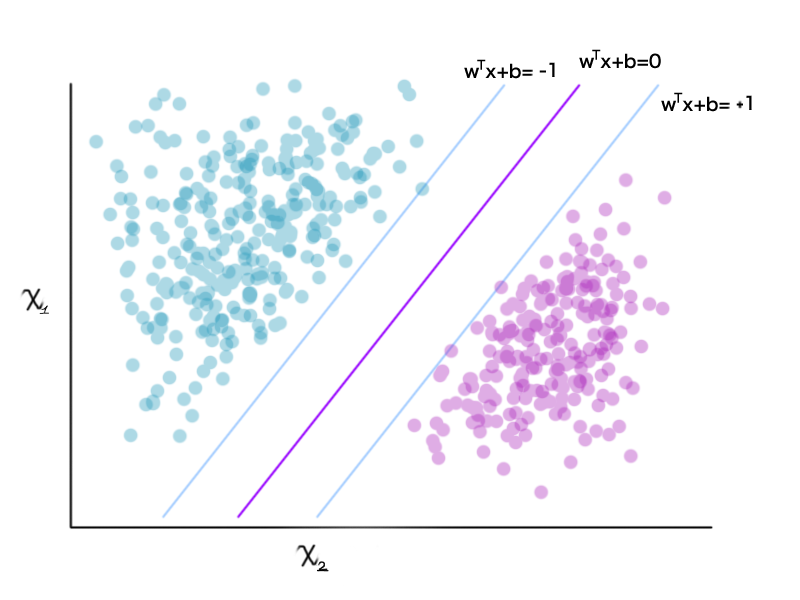
\includegraphics[width=20em]{figures/SVM_2d_example.png}
%DIFDELCMD < %%%
%DIFDELCMD < \caption{%
{%DIFAUXCMD
\DIFdelFL{Two dimensional example of an SVM classification problem}}
%DIFAUXCMD
%DIFDELCMD < \label{fig:svm}
%DIFDELCMD < \end{figure}
%DIFDELCMD < 

%DIFDELCMD < %%%
\DIFdelend In our study we used the linear kernel for our SVC\DIFdelbegin \DIFdel{, defined by the formula (\ref{eq:1}) below, where \(x\) is the input vector, \(w\) is the weight vector, and \(b\) is the bias vector. The dimensions of these vectors are such that \(f(x)\) and \(b\) are the size of the sample size, and \(w\) is the size of the amount of features. The sign of the value of \(f(x)\) determines which classification label \(y\) is applied, as shown in the formulas (\ref{eq:2}) and (\ref{eq:3})}\DIFdelend .

\DIFdelbegin \begin{displaymath}\DIFdel{%DIFDELCMD < \label{eq:1}%%%
f(x) = w^\top x + b
}\end{displaymath}
%DIFAUXCMD
\DIFdelend %DIF >  A two-dimensional example is shown in Figure \ref{fig:svm}.

\DIFdelbegin \begin{displaymath}\DIFdel{%DIFDELCMD < \label{eq:2}%%%
f(x)\geq 0 \rightarrow y= +1 
}\end{displaymath}
%DIFAUXCMD
\DIFdelend %DIF >  \begin{figure}
%DIF >  \centering
%DIF >  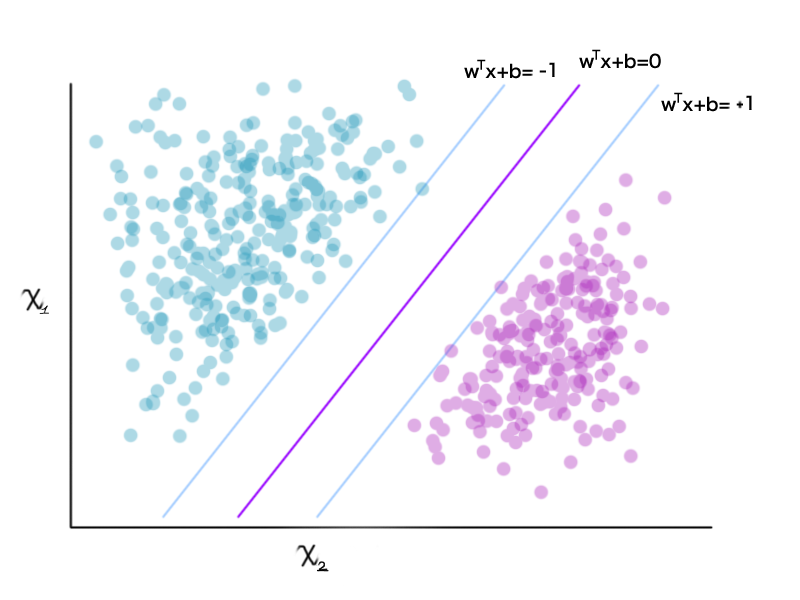
\includegraphics[width=20em]{figures/SVM_2d_example.png}
%DIF >  \caption{Two dimensional example of an SVM classification problem}
%DIF >  \label{fig:svm}
%DIF >  \end{figure}

\DIFdelbegin \begin{displaymath}\DIFdel{%DIFDELCMD < \label{eq:3}%%%
f(x)\leq 0 \rightarrow y= -1 
}\end{displaymath}
%DIFAUXCMD
%DIFDELCMD < 

%DIFDELCMD < %%%
%DIF >  In our study we used the linear kernel for our SVC, defined by the formula (\ref{eq:1}) below, where \(x\) is the input vector, \(w\) is the weight vector, and \(b\) is the bias vector. The dimensions of these vectors are such that \(f(x)\) and \(b\) are the size of the sample size, and \(w\) is the size of the amount of features. The sign of the value of \(f(x)\) determines which classification label \(y\) is applied, as shown in the formulas (\ref{eq:2}) and (\ref{eq:3}). 
\DIFaddbegin 

%DIF >  \begin{equation}\label{eq:1}
%DIF >  f(x) = w^\top x + b
%DIF >  \end{equation}

%DIF >  \begin{equation}\label{eq:2}
%DIF >  f(x)\geq 0 \rightarrow y= +1 
%DIF >  \end{equation}

%DIF >  \begin{equation}\label{eq:3}
%DIF >  f(x)\leq 0 \rightarrow y= -1 
%DIF >  \end{equation}

\DIFdel{The algorithm consists of, starting with a weight and bias vector comprised of zeroes, a randomly placed hyperplane is drawn. Each data point is tested for correct classification, and if the classification fails, the value of \(w\) is changed by a value of \(\alpha\) as follows (\ref{eq:4}) . Finally the distance to the nearest points, the support vectors, in either classification, called the margin, is calculated}\DIFdelend 

\DIFdelbegin \begin{displaymath}\DIFdel{%DIFDELCMD < \label{eq:4}%%%
w \leftarrow w + \alpha  sign(f(x_{i}))x_{i}
}\end{displaymath}
%DIFAUXCMD
\DIFdelend 

\DIFdelbegin \DIFdel{This process is repeated so that the margin is maximized and the number of erroneous classifications are minimized. 
}\DIFdelend

\subsubsection{XGBoost}
\label{xgboost}

Originally started as a research project by Tianqi Chen \cite{xgboost}, XGBoost is an improved and optimized application of a Gradient Boosting Machine, or GBM, also called gradient tree boosting, or gradient boosted regression tree. A Gradient Boosted Regression Tree (GBRT) works by building an ensemble model from several weak learning machines which are just above random guessing in accuracy, in this case using Decision Trees. The misclassified results from these weak predictions are then weighted and added to a final strong learning machine. This process iteratively optimizes the misclassification cost in a functional gradient descent so that the final learning machine focuses on important factors from the training data for a stronger prediction model. 


\DIFaddbegin \subsubsection{\DIFadd{Logistic Regression}}
\label{logit_regression}
\DIFaddend 

 \DIFaddbegin \DIFadd{The logistic model \mbox{%DIFAUXCMD
\cite{logit} }\hspace{0pt}%DIFAUXCMD
uses a logistic function to model a binary dependent variable. It is a form of regression in which the probability of the dependant variable being one of two possible values (0 or 1) is estimated from the independent variables. 
}\DIFaddend 

%DIF >  The model in its most basic form is expressed by (\ref{eq:5}), where \(p\) is the probability of the binary label being 1, \(b\) is the base of the logarithm and exponent,\(\beta_{0}\) is the y-inercept, and \(\beta_{i}\) are the coefficients for each independent variable \(x_{i}\). However, the base of the logarithm and exponent \(b\) is usually \(e\).
\DIFaddbegin 

%DIF >  \begin{equation}\label{eq:5}
%DIF >  p = \frac{1}{1+b^{-(\beta_{0}+\beta_{1}x_{1}+\beta_{2}x_{2}+ ... +\beta_{i}x_{i})}}
%DIF >  \end{equation}


\subsection{\DIFadd{Model Evaluation Metrics}}
\label{model_evaluation}

\DIFdelbegin \DIFdel{Now, in }\DIFdelend \DIFadd{In }\DIFaddend order to measure the effectiveness of the training process and data, we \DIFdelbegin \DIFdel{perform }\DIFdelend \DIFaddbegin \DIFadd{performed }\DIFaddend what is called a K-fold cross validation. This means that after randomly shuffling and splitting our training data in k equal parts, k-1 of those parts are used for training, while the remaining one part is used in validation. Using the trained \DIFdelbegin \DIFdel{SVM}\DIFdelend \DIFaddbegin \DIFadd{models}\DIFaddend , a prediction is made, and it is decided if such a prediction is correct or not, and counted and grouped as a True Positive, True Negative, False Positive or False Negative prediction. This is explained in Table \ref{tab:preds}.

\DIFdelbegin %DIFDELCMD < \begin{table} %%%
\DIFdelendFL \DIFaddbeginFL \begin{table}[htp] \DIFaddendFL \centering
\caption{Prediction outcomes}\label{tab:preds}
\begin{tabular}{|>{\centering\arraybackslash}m{7em}|>{\centering\arraybackslash}m{7em}|>{\centering\arraybackslash}m{7em}|} \arrayrulecolor{white}\hline %\cline{2-3}
\multicolumn{1}{c|}{} & \cellcolor{Mustard}\textbf{Prediction is Correct} & \cellcolor{LightPlum}\textbf{Prediction is Incorrect} \\ \hline
\cellcolor{DarkBlue}\textbf{Prediction is Positive} & \cellcolor{DeepGreen}True Positive & \cellcolor{DeepPurple}False Positive \\ \hline
\cellcolor{DeepSalmon}\textbf{Prediction is Negative} & \cellcolor{orange}True Negative & \cellcolor{Plum}False Negative \\ \hline
\end{tabular}
\end{table}

Measures of accuracy are determined from these prediction outcomes. This process is then repeated \(k\) times and the measures taken are averaged. In this study we used the \(F_{1}\) score, which measure is a harmonic mean between precision and recall. Precision, described in formula (\DIFdelbegin \DIFdel{\ref{eq:5}}\DIFdelend \DIFaddbegin \DIFadd{\ref{eq:6}}\DIFaddend ), lets us observe the rate of correct positive predictions from all the positive predictions, while Recall, detailed in formula (\DIFdelbegin \DIFdel{\ref{eq:6}}\DIFdelend \DIFaddbegin \DIFadd{\ref{eq:7}}\DIFaddend ), observes the rate of correct positive predictions from the total of actual positive data. The \(F_{1}\) score in formula (\DIFdelbegin \DIFdel{\ref{eq:7}}\DIFdelend \DIFaddbegin \DIFadd{\ref{eq:8}}\DIFaddend ) then can only be high when both of these measures are high simultaneously, and will lower substantially if they are not consistent. We use this score as it allows us to avoid overlooking data while maintaining accurate predictions.

\begin{equation}\DIFdelbegin %DIFDELCMD < \label{eq:5}
%DIFDELCMD < %%%
\DIFdelend \DIFaddbegin \label{eq:6}
\DIFaddend Precision = \frac{True Positives}{True Positives + False Positives}
\end{equation}

\begin{equation}\DIFdelbegin %DIFDELCMD < \label{eq:6}
%DIFDELCMD < %%%
\DIFdelend \DIFaddbegin \label{eq:7}
\DIFaddend Recall = \frac{True Positives}{True Positives + False Negatives}
\end{equation}

\begin{equation}\DIFdelbegin %DIFDELCMD < \label{eq:7}
%DIFDELCMD < %%%
\DIFdelend \DIFaddbegin \label{eq:8}
\DIFaddend F_{1} = 2  \frac{Precision * Recall}{Precision + Recall}
\end{equation}

\section{Experiments}
\label{experiments}

\DIFaddbegin \subsection{\DIFadd{Model Training}}
\label{model_training}

\DIFadd{As explained in section \ref{exp_design}, we designed the experiment by training variations of models depending on the input and output values. In the Tables \ref{tab:x_configurations} and \ref{tab:y_configurations}, we describe the total of different variations that we performed on each prediction model. The combinations of configurations for the input data shown were explained in Table \ref{tab:exp_var}, and they give us a total of 30,360 possible inputs for experiment variations. The possible targets explained in Tables \ref{tab:categories_ap} and \ref{tab:categories_pi} give us a total of 12 possible prediction targets. Together, we performed a total of 364,320 experiments per }\DIFaddend prediction model. \DIFaddbegin \DIFadd{Since we used 3 kinds of prediction models (SVM, XGBoost and Logistic Regression), we performed a total of 1,092,960 experiments in this study.
}\DIFaddend 


\DIFaddbegin \subsection{\DIFadd{Experiment Parameters}}
\label{params}
\DIFaddend 

 \DIFaddbegin \DIFadd{Each prediction model, SVM, XGBoost and the Logistic Regression function can have different parameters when fitting the data to the model. In this study the parameters were chosen broadly to make a general approach (not very specialized) to all the different configurations of the experiment that could take place. Because of the number of experiments explained in section \ref{model_training}, to choose parameters in a specific manner could unbalance one experiment in favor of the other. As such, we chose simple parameters that can apply to many cases.
}

\DIFadd{The SVM experiments were performed with a linear kernel and a \(C\) value of 1. The \(C\) parameter allows for misclassification in exchange of a larger margin at small values, and it becomes stricter for larger values, perhaps causing overfitting if large enough. The XGBoost experiments were performed with a learning rate of 0.1, a maximum tree depth of 3, and 100 estimators. The Logistic Regression experiments were performed with unit weight per individual sample. A 5-Fold cross validation was performed for all of the models}\DIFaddend .


\DIFdelbegin \subsection{\DIFdel{Prediction Models}}
%DIFAUXCMD
\addtocounter{subsection}{-1}%DIFAUXCMD
%DIFDELCMD < \label{pred_models}
%DIFDELCMD < %%%
\DIFdelend %DIF >  \begin{table}[p]
%DIF >  \caption{Input Data configurations}\label{tab:x_configurations}
%DIF >  \rowcolors{2}{LightPlum}{SweetPlum}
%DIF >  \begin{tabular}{|=m{5em}|+m{5em}|+l|+l|} \arrayrulecolor{white} \hline
%DIF >  \rowcolor{Plum}
%DIF >  \rowstyle{\bfseries\color{white}}
%DIF >  Prediction Model Base & Prediction Target & Input Data & Units \\ \hline
%DIF >  \begin{tabular}[c]{@{}l@{}}
%DIF >  $\bullet$ Product \\ Based \\ Model \\ \\ 
%DIF >  $\bullet$ User \\ Based \\ Model\end{tabular}
%DIF >      & \begin{tabular}[c]{@{}l@{}}
%DIF >      $\bullet$ Actual \\ Purchase\\ \\  
%DIF >      $\bullet$ Purchase \\ Intention\end{tabular} 
%DIF >          & \begin{tabular}[c]{@{}l@{}}
%DIF >          $\bullet$ Advert Viewing Time \\ Weekday Configuration\\ 
%DIF >          $\bullet$ Advert Viewing Time \\ Weekday Time Slot \\ Configuration\\ 
%DIF >          $\bullet$ Demographics (with  \\ Purchase Intention for \\ Actual Purchase)\\ 
%DIF >          $\bullet$ Advert Viewing Time \\ Weekday Configuration \\ and Demographics (with \\ Purchase Intention for \\ Actual Purchase)\\ 
%DIF >          $\bullet$ Advert Viewing Time \\ Weekday Time Slot \\ Configuration and \\ Demographics (with Purchase \\ Intention for \\ Actual Purchase)\end{tabular}
%DIF >              & \begin{tabular}[c]{@{}l@{}}
%DIF >              $\bullet$ 36 products \\ \\ 
%DIF >              $\bullet$ 3000 users \end{tabular}\\ \hline
%DIF >  \end{tabular}
%DIF >  \end{table}

\DIFdelbegin \DIFdel{Based on the input vector that is used, we have proposed investigating the two different configurations possible for our prediction models , as explained in Table \ref{tab:modelbases}.
}\DIFdelend %DIF >  \begin{table}[p] \centering
%DIF >  \caption{Possible Prediction Targets}\label{tab:y_configurations}
%DIF >  \rowcolors{2}{Liliac}{Salmon}
%DIF >  \begin{tabular}{|=c|+c|}\arrayrulecolor{white}\hline
%DIF >  \rowcolor{Plum}
%DIF >  \rowstyle{\color{white}\bfseries}
%DIF >  Prediction Targets & Number of Categories \\ \hline
%DIF >  \rowstyle{\color{black}\normalfont}
%DIF >  Actual Purchase & 6 \\ \hline
%DIF >  Purchase Intention & 6 \\ \hline
%DIF >  \end{tabular}
%DIF >  \end{table}

\DIFdelbegin %DIFDELCMD < \begin{table} \centering
%DIFDELCMD < %%%
%DIFDELCMD < \caption{%
{%DIFAUXCMD
\DIFdelFL{Prediction Model Bases}}%DIFAUXCMD
%DIFDELCMD < \label{tab:modelbases}
%DIFDELCMD < \begin{tabular}{|>{\raggedright\arraybackslash}=m{10em}|+m{22em}|} \arrayrulecolor{white}\hline
%DIFDELCMD < \rowcolor{Plum}\rowstyle{\color{white}\bfseries}
%DIFDELCMD < %%%
\DIFdelFL{Prediction Model Base }%DIFDELCMD < & %%%
\DIFdelFL{Description }%DIFDELCMD < \\ \hline
%DIFDELCMD < \rowcolor{LightBlue}
%DIFDELCMD < \pbox{10em}{\cellcolor{DarkBlue}\textbf{Product Based} \\ \textbf{Prediction Models}} & %%%
\DIFdelFL{For each product from 200 available in the survey, data from 3000 users was collected and paired with their labels. }%DIFDELCMD < \\ \hline
%DIFDELCMD < \rowcolor{LightGreen}
%DIFDELCMD < \pbox{10em}{\cellcolor{DarkLime}\textbf{User Based} \\ \textbf{Prediction Models}} & %%%
\DIFdelFL{For each user from 3000 available, data corresponding to all 200 products available in the survey was collected and paired with their labels. }%DIFDELCMD < \\ \hline
%DIFDELCMD < \end{tabular}
%DIFDELCMD < \end{table}
%DIFDELCMD < %%%
\DIFdelend 

\DIFdelbegin \DIFdel{After extracting the commercial advert viewing data using these parameters from the 3000 users that answered the survey, which includes purchase behavior questions from 200 products at two different points in time, only 38 products from those in the survey were linked to commercial adverts that were actually viewed by those same users. Thusly, we performed our experiments using the viewing data of 3000 users for these 38 products in the configurations explained before in Table \ref{tab:modelbases}}\DIFdelend


\DIFdelbegin \subsection{\DIFdel{Prediction Model Targets}}
%DIFAUXCMD
\addtocounter{subsection}{-1}%DIFAUXCMD
%DIFDELCMD < \label{pred_model_targets}
%DIFDELCMD < %%%

\DIFdelbegin \DIFdel{Using the previously explained bases, we performed analysis for both Actual Purchase and Purchase Intention, and each variation in change explained before as categories in section \ref{data_cat} of this paper. With this categorization, we can observe the difference in relation between the number of seconds of advert viewing and a change in Purchase Behavior between January 2017 and March 2017. In total we performed experiments with 24 different prediction models . This can be visualized in Table \ref{tab:experiment_models}}\DIFdelend

\section{Results}
\label{results}

 \DIFaddbegin \DIFadd{Because of the large number of experiments performed in this study, we analyze the average performances for different variations of the model input and prediction output. In order to compare the performance across different variations, we performed t-tests and examined the p-values for statistical significance. The average performance results are detailed in section \ref{av_res}. The t-test comparisons are shown in section \ref{h_res}.
}

\subsection{\DIFadd{Prediction Score Averages}}
\label{av_res}

\DIFadd{The \(F_{1}\) scores for the SVM product based model for all 36 products were averaged for each variation of the experiment. The results are shown in Table \ref{tab:svm_product_av_res}. The average \(F_{1}\) scores for the SVM user based model for all 3000 users are shown in Table \ref{tab:svm_user_av_res}.
}

\DIFadd{Similarly, the XGBoost product based models average \(F_{1}\) scores are shown in Table \ref{tab:xgboost_product_av_res}, and the user based models average \(F_{1}\) scores are shown in Table \ref{tab:xgboost_user_av_res}}.\DIFadd{Lastly, the Logistic Regression product and user based models average results are shown in Tables \ref{tab:logit_product_av_res} and \ref{tab:logit_user_av_res}.} \DIFaddend

\DIFaddbeginFL 
\begin{table}
\caption{\DIFaddFL{SVM Product Based Models Average \(F_{1}\) scores}}\label{tab:svm_product_av_res}
\resizebox{0.9\textwidth}{!}{% 
\begin{tabular}{|=l|+c|+r|+r|+r|+r|+r|+r|} \hline
\textbf{\begin{tabular}[c]{@{}l@{}}Prediction\\ Target\end{tabular}} 
    & \textbf{Category} 
    & \textbf{\begin{tabular}[c]{@{}l@{}}Advert \\ Viewing\\ Weekday \\ Time \\ Slots \end{tabular}} 
    & \textbf{\begin{tabular}[c]{@{}l@{}}Advert \\ Viewing\\ Weekday \\ Only\end{tabular}} 
    & \textbf{Demographics} 
    & \textbf{\begin{tabular}[c]{@{}l@{}}Advert \\ Viewing\\ Weekday \\ Time Slots and \\ Demographics\end{tabular}} 
    & \textbf{\begin{tabular}[c]{@{}l@{}}Advert \\ Viewing\\ Weekday \\ Only and \\ Demographics\end{tabular}} 
    & \textbf{\begin{tabular}[c]{@{}l@{}}Total \\ Average\end{tabular}} \\ \hline

\rowstyle{\bfseries}
\multirow{7}{*}{\textbf{\begin{tabular}[c]{@{}l@{}}Actual\\ Purchase\end{tabular}}}
    & \textbf{\begin{tabular}[c]{@{}l@{}}General\\ Average\end{tabular}} 
                & 0.293 & 0.292 & 0.489 & 0.495 & 0.497 & 0.413  \\ \cline{2-8} 
            & 0 & 0.000 & 0.000 & 0.211 & 0.225 & 0.218 & 0.131  \\ \cline{2-8} 
            & 1 & 0.856 & 0.852 & 0.876 & 0.878 & 0.875 & 0.867  \\ \cline{2-8} 
            & 2 & 0.000 & 0.000 & 0.327 & 0.343 & 0.343 & 0.204  \\ \cline{2-8} 
            & 3 & 0.000 & 0.000 & 0.161 & 0.171 & 0.171 & 0.102  \\ \cline{2-8} 
            & 4 & 0.000 & 0.000 & 0.446 & 0.441 & 0.441 & 0.267  \\ \cline{2-8} 
            & 5 & 0.901 & 0.900 & 0.910 & 0.911 & 0.911 & 0.907  \\ \hline

\rowstyle{\bfseries}
\multirow{7}{*}{\textbf{\begin{tabular}[c]{@{}l@{}}Purchase\\ Intention\end{tabular}}} 
    & \textbf{\begin{tabular}[c]{@{}l@{}}General\\ Average\end{tabular}} 
                & 0.252 & 0.248 & 0.273 & 0.275 & 0.276 & 0.265  \\ \cline{2-8} 
            & 0 & 0.000 & 0.000 & 0.000 & 0.000 & 0.000 & 0.000  \\ \cline{2-8} 
            & 1 & 0.570 & 0.558 & 0.590 & 0.590 & 0.596 & 0.581  \\ \cline{2-8} 
            & 2 & 0.000 & 0.000 & 0.000 & 0.000 & 0.000 & 0.000  \\ \cline{2-8} 
            & 3 & 0.115 & 0.110 & 0.139 & 0.139 & 0.138 & 0.129  \\ \cline{2-8} 
            & 4 & 0.166 & 0.156 & 0.226 & 0.226 & 0.233 & 0.202  \\ \cline{2-8} 
            & 5 & 0.662 & 0.666 & 0.685 & 0.685 & 0.689 & 0.678  \\ \hline
\rowstyle{\bfseries}
\textbf{\begin{tabular}[c]{@{}l@{}}Both \\ Targets\end{tabular}} & \textbf{\begin{tabular}[c]{@{}l@{}}Total\\ Average\end{tabular}}
                & 0.273 & 0.270 & 0.381 & 0.385 & 0.386 & 0.339  \\ \hline
\end{tabular}% 
}
\end{table}
\DIFaddendFL 
%DIF >  \end{landscape}


%DIF >  \begin{landscape}
\DIFaddbegin \begin{table}[htp] \centering
\caption{\DIFaddFL{SVM User Based Models Average \(F_{1}\) scores}}\label{tab:svm_user_av_res}
\resizebox{0.9\textwidth}{!}{% 
\begin{tabular}{|=l|+c|+r|+r|+r|+r|+r|+r|} \hline
\textbf{\begin{tabular}[c]{@{}l@{}}Prediction\\ Target\end{tabular}} 
    & \textbf{Category} 
    & \textbf{\begin{tabular}[c]{@{}l@{}}Advert \\ Viewing\\ Weekday \\ Time \\ Slots \end{tabular}} 
    & \textbf{\begin{tabular}[c]{@{}l@{}}Advert \\ Viewing\\ Weekday \\ Only\end{tabular}} 
    & \textbf{Demographics} 
    & \textbf{\begin{tabular}[c]{@{}l@{}}Advert \\ Viewing\\ Weekday \\ Time Slots and \\ Demographics\end{tabular}} 
    & \textbf{\begin{tabular}[c]{@{}l@{}}Advert \\ Viewing\\ Weekday \\ Only and \\ Demographics\end{tabular}} 
    & \textbf{\begin{tabular}[c]{@{}l@{}}Total \\ Average\end{tabular}} \\ \hline

\rowstyle{\bfseries}
\multirow{7}{*}{\textbf{\begin{tabular}[c]{@{}l@{}}Actual\\ Purchase\end{tabular}}}
    & \textbf{\begin{tabular}[c]{@{}l@{}}General\\ Average\end{tabular}} 
                & 0.317 & 0.315 & 0.391 & 0.359 & 0.373 & 0.351  \\ \cline{2-8} 
            & 0 & 0.055 & 0.049 & 0.095 & 0.085 & 0.087 & 0.074  \\ \cline{2-8} 
            & 1 & 0.745 & 0.755 & 0.854 & 0.789 & 0.812 & 0.791  \\ \cline{2-8} 
            & 2 & 0.074 & 0.070 & 0.140 & 0.114 & 0.126 & 0.105  \\ \cline{2-8} 
            & 3 & 0.076 & 0.071 & 0.108 & 0.107 & 0.121 & 0.096  \\ \cline{2-8} 
            & 4 & 0.140 & 0.126 & 0.254 & 0.221 & 0.239 & 0.196  \\ \cline{2-8} 
            & 5 & 0.812 & 0.822 & 0.893 & 0.840 & 0.855 & 0.844  \\ \hline

\rowstyle{\bfseries}
\multirow{7}{*}{\textbf{\begin{tabular}[c]{@{}l@{}}Purchase\\ Intention\end{tabular}}} 
    & \textbf{\begin{tabular}[c]{@{}l@{}}General\\ Average\end{tabular}} 
                & 0.297 & 0.289 & 0.242 & 0.296 & 0.290 & 0.283  \\ \cline{2-8} 
            & 0 & 0.036 & 0.032 & 0.006 & 0.036 & 0.033 & 0.029  \\ \cline{2-8} 
            & 1 & 0.553 & 0.553 & 0.534 & 0.548 & 0.553 & 0.548  \\ \cline{2-8} 
            & 2 & 0.048 & 0.043 & 0.007 & 0.049 & 0.042 & 0.038  \\ \cline{2-8} 
            & 3 & 0.217 & 0.195 & 0.093 & 0.217 & 0.198 & 0.184  \\ \cline{2-8} 
            & 4 & 0.301 & 0.279 & 0.174 & 0.299 & 0.280 & 0.267  \\ \cline{2-8} 
            & 5 & 0.629 & 0.634 & 0.639 & 0.626 & 0.632 & 0.632  \\ \hline
\rowstyle{\bfseries}
\textbf{\begin{tabular}[c]{@{}l@{}}Both \\ Targets\end{tabular}} & \textbf{\begin{tabular}[c]{@{}l@{}}Total\\ Average\end{tabular}}
                & 0.307 & 0.302 & 0.316 & 0.327 & 0.331 & 0.317  \\ \hline
\end{tabular}% 
}
\end{table}
%DIF >  \end{landscape}
\DIFaddend 

%%%%%%%%%%%%%%%%%%
%%%% XGBoost %%%%%
%%%%%%%%%%%%%%%%%%

%DIF >  \begin{landscape}
\DIFaddbeginFL 
\begin{table}[htp] \centering
\caption{\DIFaddFL{XGBoost Product Based Models Average \(F_{1}\) scores}}\label{tab:xgboost_product_av_res}
\resizebox{0.9\textwidth}{!}{% 
\begin{tabular}{|=l|+c|+r|+r|+r|+r|+r|+r|} \hline
\textbf{\begin{tabular}[c]{@{}l@{}}Prediction\\ Target\end{tabular}} 
    & \textbf{Category} 
    & \textbf{\begin{tabular}[c]{@{}l@{}}Advert \\ Viewing\\ Weekday \\ Time \\ Slots \end{tabular}} 
    & \textbf{\begin{tabular}[c]{@{}l@{}}Advert \\ Viewing\\ Weekday \\ Only\end{tabular}} 
    & \textbf{Demographics} 
    & \textbf{\begin{tabular}[c]{@{}l@{}}Advert \\ Viewing\\ Weekday \\ Time Slots and \\ Demographics\end{tabular}} 
    & \textbf{\begin{tabular}[c]{@{}l@{}}Advert \\ Viewing\\ Weekday \\ Only and \\ Demographics\end{tabular}} 
    & \textbf{\begin{tabular}[c]{@{}l@{}}Total \\ Average\end{tabular}} \\ \hline

\rowstyle{\bfseries}
\multirow{7}{*}{\textbf{\begin{tabular}[c]{@{}l@{}}Actual\\ Purchase\end{tabular}}}
    & \textbf{\begin{tabular}[c]{@{}l@{}}General\\ Average\end{tabular}} 
                & 0.293 & 0.294 & 0.307 & 0.309 & 0.308 & 0.302  \\ \cline{2-8} 
            & 0 & 0.001 & 0.000 & 0.027 & 0.030 & 0.029 & 0.017  \\ \cline{2-8} 
            & 1 & 0.847 & 0.849 & 0.756 & 0.755 & 0.752 & 0.792  \\ \cline{2-8} 
            & 2 & 0.001 & 0.000 & 0.048 & 0.054 & 0.052 & 0.031  \\ \cline{2-8} 
            & 3 & 0.003 & 0.003 & 0.043 & 0.044 & 0.045 & 0.028  \\ \cline{2-8} 
            & 4 & 0.008 & 0.010 & 0.136 & 0.136 & 0.133 & 0.085  \\ \cline{2-8} 
            & 5 & 0.898 & 0.900 & 0.835 & 0.835 & 0.833 & 0.860  \\ \hline

\rowstyle{\bfseries}
\multirow{7}{*}{\textbf{\begin{tabular}[c]{@{}l@{}}Purchase\\ Intention\end{tabular}}} 
    & \textbf{\begin{tabular}[c]{@{}l@{}}General\\ Average\end{tabular}} 
                & 0.257 & 0.257 & 0.266 & 0.266 & 0.268 & 0.263  \\ \cline{2-8} 
            & 0 & 0.000 & 0.000 & 0.000 & 0.002 & 0.001 & 0.001  \\ \cline{2-8} 
            & 1 & 0.574 & 0.571 & 0.573 & 0.565 & 0.572 & 0.571  \\ \cline{2-8} 
            & 2 & 0.000 & 0.001 & 0.001 & 0.001 & 0.002 & 0.001  \\ \cline{2-8} 
            & 3 & 0.121 & 0.122 & 0.136 & 0.136 & 0.142 & 0.131  \\ \cline{2-8} 
            & 4 & 0.175 & 0.175 & 0.211 & 0.220 & 0.219 & 0.200  \\ \cline{2-8} 
            & 5 & 0.670 & 0.674 & 0.673 & 0.669 & 0.674 & 0.672  \\ \hline
\rowstyle{\bfseries}
\textbf{\begin{tabular}[c]{@{}l@{}}Both \\ Targets\end{tabular}} & \textbf{\begin{tabular}[c]{@{}l@{}}Total\\ Average\end{tabular}}
                & 0.275 & 0.275 & 0.287 & 0.287 & 0.288 & 0.282  \\ \hline
\end{tabular}% 
}
\end{table}
%DIF >  \end{landscape}
\DIFaddendFL

%DIF >  \begin{landscape}
\DIFaddbegin \begin{table}[htp] \centering
\caption{\DIFaddFL{XGBoost User Based Models Average \(F_{1}\) scores}}\label{tab:xgboost_user_av_res}
\resizebox{0.9\textwidth}{!}{% 
\begin{tabular}{|=l|+c|+r|+r|+r|+r|+r|+r|} \hline
\textbf{\begin{tabular}[c]{@{}l@{}}Prediction\\ Target\end{tabular}} 
    & \textbf{Category} 
    & \textbf{\begin{tabular}[c]{@{}l@{}}Advert \\ Viewing\\ Weekday \\ Time \\ Slots \end{tabular}} 
    & \textbf{\begin{tabular}[c]{@{}l@{}}Advert \\ Viewing\\ Weekday \\ Only\end{tabular}} 
    & \textbf{Demographics} 
    & \textbf{\begin{tabular}[c]{@{}l@{}}Advert \\ Viewing\\ Weekday \\ Time Slots and \\ Demographics\end{tabular}} 
    & \textbf{\begin{tabular}[c]{@{}l@{}}Advert \\ Viewing\\ Weekday \\ Only and \\ Demographics\end{tabular}} 
    & \textbf{\begin{tabular}[c]{@{}l@{}}Total \\ Average\end{tabular}} \\ \hline

\rowstyle{\bfseries}
\multirow{7}{*}{\textbf{\begin{tabular}[c]{@{}l@{}}Actual\\ Purchase\end{tabular}}}
    & \textbf{\begin{tabular}[c]{@{}l@{}}General\\ Average\end{tabular}} 
                & 0.291 & 0.291 & 0.297 & 0.301 & 0.302 & 0.296  \\ \cline{2-8} 
            & 0 & 0.008 & 0.008 & 0.018 & 0.021 & 0.021 & 0.015  \\ \cline{2-8} 
            & 1 & 0.771 & 0.769 & 0.752 & 0.758 & 0.760 & 0.762  \\ \cline{2-8} 
            & 2 & 0.014 & 0.014 & 0.030 & 0.032 & 0.033 & 0.025  \\ \cline{2-8} 
            & 3 & 0.027 & 0.029 & 0.042 & 0.048 & 0.049 & 0.039  \\ \cline{2-8} 
            & 4 & 0.082 & 0.084 & 0.119 & 0.121 & 0.123 & 0.106  \\ \cline{2-8} 
            & 5 & 0.841 & 0.842 & 0.825 & 0.827 & 0.825 & 0.832  \\ \hline

\rowstyle{\bfseries}
\multirow{7}{*}{\textbf{\begin{tabular}[c]{@{}l@{}}Purchase\\ Intention\end{tabular}}} 
    & \textbf{\begin{tabular}[c]{@{}l@{}}General\\ Average\end{tabular}} 
                & 0.267 & 0.269 & 0.239 & 0.267 & 0.268 & 0.262  \\ \cline{2-8} 
            & 0 & 0.008 & 0.008 & 0.001 & 0.008 & 0.007 & 0.006  \\ \cline{2-8} 
            & 1 & 0.538 & 0.543 & 0.533 & 0.542 & 0.542 & 0.540  \\ \cline{2-8} 
            & 2 & 0.013 & 0.013 & 0.001 & 0.013 & 0.013 & 0.010  \\ \cline{2-8} 
            & 3 & 0.154 & 0.161 & 0.085 & 0.155 & 0.159 & 0.143  \\ \cline{2-8} 
            & 4 & 0.249 & 0.250 & 0.174 & 0.248 & 0.252 & 0.235  \\ \cline{2-8} 
            & 5 & 0.638 & 0.637 & 0.643 & 0.636 & 0.636 & 0.638  \\ \hline

\rowstyle{\bfseries}
\textbf{\begin{tabular}[c]{@{}l@{}}Both \\ Targets\end{tabular}} & \textbf{\begin{tabular}[c]{@{}l@{}}Total\\ Average\end{tabular}}
                & 0.279 & 0.280 & 0.268 & 0.284 & 0.285 & 0.279  \\ \hline
\end{tabular}% 
}
\end{table}
%DIF >  \end{landscape}


%DIF > %%%%%%%%%%%%%%%%%
%DIF > %%%% Logit  %%%%%
%DIF > %%%%%%%%%%%%%%%%%

%DIF >  \begin{landscape}
\begin{table}[htp] \centering
\caption{\DIFaddFL{Logistic Regression Product Based Models Average \(F_{1}\) scores}}\label{tab:logit_product_av_res}
\resizebox{0.9\textwidth}{!}{% 
\begin{tabular}{|=l|+c|+r|+r|+r|+r|+r|+r|} \hline
\textbf{\begin{tabular}[c]{@{}l@{}}Prediction\\ Target\end{tabular}} 
    & \textbf{Category} 
    & \textbf{\begin{tabular}[c]{@{}l@{}}Advert \\ Viewing\\ Weekday \\ Time \\ Slots \end{tabular}} 
    & \textbf{\begin{tabular}[c]{@{}l@{}}Advert \\ Viewing\\ Weekday \\ Only\end{tabular}} 
    & \textbf{Demographics} 
    & \textbf{\begin{tabular}[c]{@{}l@{}}Advert \\ Viewing\\ Weekday \\ Time Slots and \\ Demographics\end{tabular}} 
    & \textbf{\begin{tabular}[c]{@{}l@{}}Advert \\ Viewing\\ Weekday \\ Only and \\ Demographics\end{tabular}} 
    & \textbf{\begin{tabular}[c]{@{}l@{}}Total \\ Average\end{tabular}} \\ \hline

\rowstyle{\bfseries}
\multirow{7}{*}{\textbf{\begin{tabular}[c]{@{}l@{}}Actual\\ Purchase\end{tabular}}}
    & \textbf{\begin{tabular}[c]{@{}l@{}}General\\ Average\end{tabular}} 
                & 0.293 & 0.293 & 0.500 & 0.513 & 0.508 & 0.421  \\ \cline{2-8} 
            & 0 & 0.000 & 0.000 & 0.226 & 0.234 & 0.237 & 0.139  \\ \cline{2-8} 
            & 1 & 0.851 & 0.853 & 0.874 & 0.874 & 0.875 & 0.865  \\ \cline{2-8} 
            & 2 & 0.000 & 0.000 & 0.343 & 0.368 & 0.355 & 0.213  \\ \cline{2-8} 
            & 3 & 0.002 & 0.000 & 0.181 & 0.208 & 0.195 & 0.117  \\ \cline{2-8} 
            & 4 & 0.006 & 0.004 & 0.462 & 0.480 & 0.475 & 0.286  \\ \cline{2-8} 
            & 5 & 0.899 & 0.901 & 0.914 & 0.914 & 0.914 & 0.909  \\ \hline

\rowstyle{\bfseries}
\multirow{7}{*}{\textbf{\begin{tabular}[c]{@{}l@{}}Purchase\\ Intention\end{tabular}}} 
    & \textbf{\begin{tabular}[c]{@{}l@{}}General\\ Average\end{tabular}} 
                & 0.259 & 0.256 & 0.289 & 0.294 & 0.292 & 0.278  \\ \cline{2-8} 
            & 0 & 0.000 & 0.000 & 0.000 & 0.000 & 0.000 & 0.000  \\ \cline{2-8} 
            & 1 & 0.575 & 0.572 & 0.608 & 0.611 & 0.611 & 0.595  \\ \cline{2-8} 
            & 2 & 0.000 & 0.000 & 0.000 & 0.001 & 0.000 & 0.000  \\ \cline{2-8} 
            & 3 & 0.125 & 0.118 & 0.159 & 0.170 & 0.163 & 0.147  \\ \cline{2-8} 
            & 4 & 0.184 & 0.174 & 0.270 & 0.280 & 0.278 & 0.237  \\ \cline{2-8} 
            & 5 & 0.671 & 0.668 & 0.696 & 0.703 & 0.701 & 0.688  \\ \hline
\rowstyle{\bfseries}
\textbf{\begin{tabular}[c]{@{}l@{}}Both \\ Targets\end{tabular}} & \textbf{\begin{tabular}[c]{@{}l@{}}Total\\ Average\end{tabular}}
                & 0.276 & 0.274 & 0.394 & 0.404 & 0.400 & 0.350  \\ \hline
\end{tabular}% 
}
\end{table}
%DIF >  \end{landscape}

%DIF >  \begin{landscape}
\begin{table}[htp] \centering
\caption{\DIFaddFL{Logistic Regression User Based Models Average \(F_{1}\) scores}}\label{tab:logit_user_av_res}
\resizebox{0.9\textwidth}{!}{% 
\begin{tabular}{|=l|+c|+r|+r|+r|+r|+r|+r|} \hline
\textbf{\begin{tabular}[c]{@{}l@{}}Prediction\\ Target\end{tabular}} 
    & \textbf{Category} 
    & \textbf{\begin{tabular}[c]{@{}l@{}}Advert \\ Viewing\\ Weekday \\ Time \\ Slots \end{tabular}} 
    & \textbf{\begin{tabular}[c]{@{}l@{}}Advert \\ Viewing\\ Weekday \\ Only\end{tabular}} 
    & \textbf{Demographics} 
    & \textbf{\begin{tabular}[c]{@{}l@{}}Advert \\ Viewing\\ Weekday \\ Time Slots and \\ Demographics\end{tabular}} 
    & \textbf{\begin{tabular}[c]{@{}l@{}}Advert \\ Viewing\\ Weekday \\ Only and \\ Demographics\end{tabular}} 
    & \textbf{\begin{tabular}[c]{@{}l@{}}Total \\ Average\end{tabular}} \\ \hline

\rowstyle{\bfseries}
\multirow{7}{*}{\textbf{\begin{tabular}[c]{@{}l@{}}Actual\\ Purchase\end{tabular}}}
    & \textbf{\begin{tabular}[c]{@{}l@{}}General\\ Average\end{tabular}} 
                & 0.312 & 0.309 & 0.347 & 0.333 & 0.341 & 0.328  \\ \cline{2-8} 
            & 0 & 0.046 & 0.040 & 0.037 & 0.056 & 0.054 & 0.047  \\ \cline{2-8} 
            & 1 & 0.740 & 0.750 & 0.846 & 0.771 & 0.794 & 0.780  \\ \cline{2-8} 
            & 2 & 0.064 & 0.058 & 0.070 & 0.083 & 0.082 & 0.071  \\ \cline{2-8} 
            & 3 & 0.074 & 0.066 & 0.064 & 0.089 & 0.091 & 0.077  \\ \cline{2-8} 
            & 4 & 0.139 & 0.124 & 0.175 & 0.173 & 0.185 & 0.159  \\ \cline{2-8} 
            & 5 & 0.806 & 0.815 & 0.888 & 0.827 & 0.844 & 0.836  \\ \hline

\rowstyle{\bfseries}
\multirow{7}{*}{\textbf{\begin{tabular}[c]{@{}l@{}}Purchase\\ Intention\end{tabular}}} 
    & \textbf{\begin{tabular}[c]{@{}l@{}}General\\ Average\end{tabular}} 
                & 0.298 & 0.295 & 0.242 & 0.298 & 0.293 & 0.285  \\ \cline{2-8} 
            & 0 & 0.037 & 0.035 & 0.007 & 0.038 & 0.034 & 0.030  \\ \cline{2-8} 
            & 1 & 0.555 & 0.557 & 0.535 & 0.554 & 0.556 & 0.551  \\ \cline{2-8} 
            & 2 & 0.052 & 0.047 & 0.009 & 0.052 & 0.044 & 0.041  \\ \cline{2-8} 
            & 3 & 0.220 & 0.204 & 0.093 & 0.220 & 0.207 & 0.189  \\ \cline{2-8} 
            & 4 & 0.298 & 0.288 & 0.175 & 0.300 & 0.286 & 0.269  \\ \cline{2-8} 
            & 5 & 0.628 & 0.635 & 0.636 & 0.628 & 0.634 & 0.632  \\ \hline
\rowstyle{\bfseries}
\textbf{\begin{tabular}[c]{@{}l@{}}Both \\ Targets\end{tabular}} & \textbf{\begin{tabular}[c]{@{}l@{}}Total\\ Average\end{tabular}}
                & 0.305 & 0.302 & 0.294 & 0.316 & 0.317 & 0.307  \\ \hline
\end{tabular}% 
}
\end{table}
%DIF >  \end{landscape}


\subsection{\DIFadd{Statistical Analysis}}
\label{h_res}


\DIFadd{In this study we performed a series of experiments where we trained different prediction models based on either advert viewing time or demographic data to predict purchase behaviors of actual purchase and purchase intention across 3000 users and 36 products. If we were able to predict purchase behaviors with models based on exposure time more reliably than with models based on demographic data, obvious strategy for businesses would be to increase the number of adverts. On the other hand, if models based on exposure time had unreliable predictability in contrast to models based on demographic data, doubts would surface about the hard investment in television advertising. 
}

\DIFadd{In order to analyze the change in predictability of purchase behavior we averaged the }\DIFaddend results \DIFdelbegin \DIFdel{for SVM and XGBoost experiments in a later section}\DIFdelend \DIFaddbegin \DIFadd{of predictions across different variations of the experiments, detailed in the previous section, and then performed t-tests to observe the difference in performance between sets of results. We established 3 hypotheses to test for, explained below}\DIFaddend .

\DIFaddbegin \begin{hyp}
\label{hyp:1}
\DIFadd{Advert viewing time based models perform differently from demographics based models.
}\end{hyp}
\DIFaddend 

\DIFaddbegin \DIFadd{For this hypothesis, we performed a t-test bewteen the results from models that include advert viewing time and the models that only include demographic data. More specifically, we tested the Weekday Time Slot model results against the Demographics models, and the Weekday Only models against the Demographics models. The p-values for each t-test are shown in Table \ref{tab:h1_ap} for Actual Purchase predictions and in Table \ref{tab:h1_pi} for Purchase Intention predictions. With these tests, we will examine the changes in predictability against demographic data, which we are using as the control data for our experiments. This will allow us to determine whether the advert viewing time based models are performing better or worse than the demographic models, and therefore conclude whether the advert viewing time is having an effect on customers purchase behavior or if it is decided by external factors}\DIFaddend .

%DIF > %% Actual Purchase
\DIFaddbegin \begin{table}[p] \centering
\caption{\DIFaddFL{Hypothesis 1 t-test: p-values for Actual Purchase behavior}}\label{tab:h1_ap}
\resizebox{1\textwidth}{!}{% 
\begin{tabular}{|c|c|l|r|r|r|r|r|r|}
\hline
\multirow{2}{*}{\textbf{Model}} 
    & \multirow{2}{*}{\textbf{Base}} 
    & \multicolumn{1}{c|}{\multirow{2}{*}{\textbf{Configuration}}} 
    & \multicolumn{6}{c|}{\textbf{Actual Purchase Categories}} \\ \cline{4-9} 
    & & \multicolumn{1}{c|}{}
      & \multicolumn{1}{c|}{\textbf{0}} 
      & \multicolumn{1}{c|}{\textbf{1}} 
      & \multicolumn{1}{c|}{\textbf{2}} 
      & \multicolumn{1}{c|}{\textbf{3}} 
      & \multicolumn{1}{c|}{\textbf{4}} 
      & \multicolumn{1}{c|}{\textbf{5}} \\ \hline
\multirow{4}{*}{SVM} 
    & \multirow{2}{*}{product} 
        & Weekday Time Slot     & 0.000 & 0.328 & 0.000 & 0.001 & 0.000 & 0.567 \\ \cline{3-9} 
      & & Weekday Only              & 0.000 & 0.284 & 0.000 & 0.001 & 0.000 & 0.527 \\ \cline{2-9} 
    & \multirow{2}{*}{user} 
        & Weekday Time Slot     & 0.000 & 0.000 & 0.000 & 0.000 & 0.000 & 0.000 \\ \cline{3-9} 
      & & Weekday Only              & 0.000 & 0.000 & 0.000 & 0.000 & 0.000 & 0.000 \\ \hline
\multirow{4}{*}{XGBoost}
    & \multirow{2}{*}{product} 
        & Weekday Time Slot     & 0.000 & 0.005 & 0.000 & 0.015 & 0.000 & 0.013 \\ \cline{3-9} 
      & & Weekday Only              & 0.000 & 0.004 & 0.000 & 0.015 & 0.000 & 0.011 \\ \cline{2-9} 
    & \multirow{2}{*}{user}    
        & Weekday Time Slot     & 0.000 & 0.004 & 0.000 & 0.000 & 0.000 & 0.004 \\ \cline{3-9} 
      & & Weekday Only              & 0.000 & 0.010 & 0.000 & 0.000 & 0.000 & 0.003 \\ \hline
\multirow{4}{*}{\begin{tabular}[c]{@{}c@{}}Logistic \\ Regression\end{tabular}} 
    & \multirow{2}{*}{product} 
        & Weekday Time Slot     & 0.000 & 0.282 & 0.000 & 0.000 & 0.000 & 0.348 \\ \cline{3-9} 
      & & Weekday Only              & 0.000 & 0.327 & 0.000 & 0.000 & 0.000 & 0.414 \\ \cline{2-9} 
    & \multirow{2}{*}{user} 
        & Weekday Time Slot     & 0.012 & 0.000 & 0.236 & 0.032 & 0.000 & 0.000 \\ \cline{3-9} 
      & & Weekday Only              & 0.374 & 0.000 & 0.007 & 0.757 & 0.000 & 0.000 \\ \hline
\end{tabular}% 
}
\end{table}
\DIFaddend 

 %DIF > %% Purchase Intention
\DIFaddbegin \begin{table}[p] \centering
\caption{\DIFaddFL{Hypothesis 1 t-test: p-values for Purchase Intention behavior}}\label{tab:h1_pi}
\resizebox{1\textwidth}{!}{% 
\begin{tabular}{|c|c|l|r|r|r|r|r|r|}
\hline
\multirow{2}{*}{\textbf{Model}} 
    & \multirow{2}{*}{\textbf{Base}} 
    & \multicolumn{1}{c|}{\multirow{2}{*}{\textbf{Configuration}}} 
    & \multicolumn{6}{c|}{\textbf{Purchase Intention Categories}} \\ \cline{4-9} 
    & & \multicolumn{1}{c|}{}
      & \multicolumn{1}{c|}{\textbf{0}} 
      & \multicolumn{1}{c|}{\textbf{1}} 
      & \multicolumn{1}{c|}{\textbf{2}} 
      & \multicolumn{1}{c|}{\textbf{3}} 
      & \multicolumn{1}{c|}{\textbf{4}} 
      & \multicolumn{1}{c|}{\textbf{5}} \\ \hline
\multirow{4}{*}{SVM}
    & \multirow{2}{*}{product} 
        & Weekday Time Slot     & nan   & 0.803 & nan   & 0.700 & 0.405 & 0.767 \\ \cline{3-9} 
      & & Weekday Only              & nan   & 0.694 & nan   & 0.644 & 0.329 & 0.808 \\ \cline{2-9} 
    & \multirow{2}{*}{user}
        & Weekday Time Slot     & 0.000 & 0.026 & 0.000 & 0.000 & 0.000 & 0.234 \\ \cline{3-9} 
      & & Weekday Only              & 0.000 & 0.028 & 0.000 & 0.000 & 0.000 & 0.534 \\ \hline
\multirow{4}{*}{XGBoost}
    & \multirow{2}{*}{product}
        & Weekday Time Slot     & 0.324 & 0.983 & 0.041 & 0.804 & 0.598 & 0.969 \\ \cline{3-9} 
      & & Weekday Only              & 0.324 & 0.982 & 0.203 & 0.811 & 0.606 & 0.992 \\ \cline{2-9} 
    & \multirow{2}{*}{user}
        & Weekday Time Slot     & 0.000 & 0.533 & 0.000 & 0.000 & 0.000 & 0.585 \\ \cline{3-9} 
      & & Weekday Only              & 0.000 & 0.246 & 0.000 & 0.000 & 0.000 & 0.509 \\ \hline
\multirow{4}{*}{\begin{tabular}[c]{@{}c@{}}Logistic \\ Regression\end{tabular}}
    & \multirow{2}{*}{product}
        & Weekday Time Slot     & nan   & 0.673 & 0.803 & 0.582 & 0.222 & 0.724 \\ \cline{3-9} 
      & & Weekday Only              & nan   & 0.655 & 0.324 & 0.514 & 0.175 & 0.704 \\ \cline{2-9} 
    & \multirow{2}{*}{user}
        & Weekday Time Slot     & 0.000 & 0.017 & 0.000 & 0.000 & 0.000 & 0.364 \\ \cline{3-9} 
      & & Weekday Only              & 0.000 & 0.010 & 0.000 & 0.000 & 0.000 & 0.947 \\ \hline
\end{tabular}% 
}
\end{table}
\DIFaddend 

\DIFaddbegin \begin{hyp}
\label{hyp:2}
\DIFadd{Demographic and advert viewing based models perform differently from demographic based models.
}\end{hyp}
\DIFaddend 

\DIFaddbegin \DIFadd{For this hypothesis, we performed a t-test bewteen the results from models that include both advert viewing time and demographich data, and the models that only include demographic data. More specifically, we tested the Weekday Time Slot and Demographics model results against the Demographics models, and the Weekday and Demographics models against the Demographics models. The p-values for each t-test are shown in Table \ref{tab:h2_ap} for Actual Purchase predictions and in Table \ref{tab:h2_pi} for Purchase Intention predictions. With these tests, we will examine if adding the advert viewing data to the demographic data causes any major changes, to determine if the predictions are being improved, worsened, or if they stay the same regardless of advert viewing}\DIFaddend .

\DIFaddbeginFL 
\begin{table}
\caption{\DIFaddFL{Hypothesis 2 t-test: p-values for Actual Purchase behavior}}\label{tab:h2_ap}
\resizebox{\textwidth}{!}{%
\begin{tabular}{|c|c|l|r|r|r|r|r|r|}
\hline
\multirow{2}{*}{\textbf{Model}} 
    & \multirow{2}{*}{\textbf{Base}} 
    & \multicolumn{1}{c|}{\multirow{2}{*}{\textbf{Configuration}}} 
    & \multicolumn{6}{c|}{\textbf{Actual Purchase Categories}} \\ \cline{4-9} 
    & & \multicolumn{1}{c|}{}
      & \multicolumn{1}{c|}{\textbf{0}} 
      & \multicolumn{1}{c|}{\textbf{1}} 
      & \multicolumn{1}{c|}{\textbf{2}} 
      & \multicolumn{1}{c|}{\textbf{3}} 
      & \multicolumn{1}{c|}{\textbf{4}} 
      & \multicolumn{1}{c|}{\textbf{5}} \\ \hline
\multirow{4}{*}{SVM} 
    & \multirow{2}{*}{product} 
        & Weekday Time Slot     & 0.923 & 0.953 & 0.748 & 0.777 & 0.968 & 0.980 \\ \cline{3-9} 
      & & Weekday Only              & 0.850 & 0.936 & 0.839 & 0.868 & 0.942 & 0.956 \\ \cline{2-9} 
 & \multirow{2}{*}{user} 
    & Weekday Time Slot         & 0.056 & 0.000 & 0.000 & 0.837 & 0.000 & 0.000 \\ \cline{3-9} 
      & & Weekday Only              & 0.139 & 0.000 & 0.033 & 0.038 & 0.078 & 0.000 \\ \hline
\multirow{4}{*}{XGBoost} 
    & \multirow{2}{*}{product} 
        & Weekday Time Slot     & 0.758 & 0.973 & 0.581 & 0.936 & 0.991 & 0.993 \\ \cline{3-9} 
      & & Weekday Only              & 0.811 & 0.929 & 0.703 & 0.897 & 0.924 & 0.956 \\ \cline{2-9} 
 & \multirow{2}{*}{user} 
    & Weekday Time Slot         & 0.074 & 0.318 & 0.413 & 0.057 & 0.625 & 0.655 \\ \cline{3-9} 
      & & Weekday Only              & 0.069 & 0.187 & 0.173 & 0.045 & 0.388 & 0.993 \\ \hline
\multirow{4}{*}{\begin{tabular}[c]{@{}c@{}}Logistic \\ Regression\end{tabular}} 
    & \multirow{2}{*}{product} 
        & Weekday Time Slot     & 0.894 & 0.997 & 0.674 & 0.627 & 0.772 & 0.971 \\ \cline{3-9} 
      & & Weekday Only              & 0.856 & 0.955 & 0.846 & 0.808 & 0.831 & 0.990 \\ \cline{2-9} 
 & \multirow{2}{*}{user} 
    & Weekday Time Slot         & 0.000 & 0.000 & 0.007 & 0.000 & 0.823 & 0.000 \\ \cline{3-9} 
      & & Weekday Only              & 0.000 & 0.000 & 0.017 & 0.000 & 0.187 & 0.000 \\ \hline
\end{tabular}%
}
\DIFaddendFL \end{table}

%% Purchase Intention
\DIFaddbegin \begin{table}[p] \centering
\caption{\DIFaddFL{Hypothesis 2 t-test: p-values for Purchase Intention behavior}}\label{tab:h2_pi}
\resizebox{\textwidth}{!}{%
\begin{tabular}{|c|c|l|r|r|r|r|r|r|}
\hline
\multirow{2}{*}{\textbf{Model}} 
    & \multirow{2}{*}{\textbf{Base}} 
    & \multicolumn{1}{c|}{\multirow{2}{*}{\textbf{Configuration}}} 
    & \multicolumn{6}{c|}{\textbf{Purchase Intention Categories}} \\ \cline{4-9} 
    & & \multicolumn{1}{c|}{}
      & \multicolumn{1}{c|}{\textbf{0}} 
      & \multicolumn{1}{c|}{\textbf{1}} 
      & \multicolumn{1}{c|}{\textbf{2}} 
      & \multicolumn{1}{c|}{\textbf{3}} 
      & \multicolumn{1}{c|}{\textbf{4}} 
      & \multicolumn{1}{c|}{\textbf{5}} \\ \hline
\multirow{4}{*}{SVM} 
    & \multirow{2}{*}{product} 
        & Weekday Time Slot      & nan & 0.942 & nan & 0.985 & 0.930 & 0.969 \\ \cline{3-9} 
      & & Weekday Only               & nan & 0.986 & nan & 0.991 & 0.950 & 0.955 \\ \cline{2-9} 
    & \multirow{2}{*}{user} 
        & Weekday Time Slot      & 0.000 & 0.099 & 0.000 & 0.000 & 0.000 & 0.118 \\ \cline{3-9} 
      & & Weekday Only               & 0.000 & 0.029 & 0.000 & 0.000 & 0.000 & 0.402 \\ \hline
\multirow{4}{*}{XGBoost} 
    & \multirow{2}{*}{product} 
        & Weekday Time Slot      & 0.002 & 0.924 & 0.850 & 0.996 & 0.900 & 0.960 \\ \cline{3-9} 
      & & Weekday Only               & 0.115 & 0.990 & 0.364 & 0.916 & 0.916 & 0.986 \\ \cline{2-9} 
    & \multirow{2}{*}{user} 
        & Weekday Time Slot      & 0.000 & 0.290 & 0.000 & 0.000 & 0.000 & 0.409 \\ \cline{3-9} 
      & & Weekday Only               & 0.000 & 0.303 & 0.000 & 0.000 & 0.000 & 0.400 \\ \hline
\multirow{4}{*}{\begin{tabular}[c]{@{}c@{}}Logistic \\ Regression\end{tabular}} 
    & \multirow{2}{*}{product} 
        & Weekday Time Slot      & nan & 0.957 & 0.331 & 0.856 & 0.884 & 0.916 \\ \cline{3-9} 
      & & Weekday Only               & nan & 0.957 & 0.871 & 0.943 & 0.903 & 0.943 \\ \cline{2-9} 
    & \multirow{2}{*}{user} 
        & Weekday Time Slot      & 0.000 & 0.028 & 0.000 & 0.000 & 0.000 & 0.313 \\ \cline{3-9} 
      & & Weekday Only               & 0.000 & 0.016 & 0.000 & 0.000 & 0.000 & 0.869 \\ \hline
\end{tabular}%
}
\end{table}
\DIFaddend 

\DIFaddbegin \begin{hyp}
\label{hyp:3}
\DIFadd{Advert viewing time based models perform differently from demographic and advert viewing based models.
}\end{hyp}
\DIFaddend 

\DIFaddbegin \DIFadd{For this hypothesis, we performed a t-test bewteen the results from models that include both advert viewing time and demographich data, and the models that only include advert viewing data. More specifically, we tested the Weekday Time Slot and Demographics model results against the Weekday Time Slot models, and the Weekday and Demographics models against the Weekday Only models. The p-values for each t-test are shown in Table \ref{tab:h3_ap} for Actual Purchase predictions and in Table \ref{tab:h3_pi} for Purchase Intention predictions. With these tests, we will examine if adding the demographic data to the advert viewing data causes any major changes, to determine if the predictions are being improved, worsened or if they stay the same regardless of demographic variances. By performing this last test, as well as the differences tested by Hypothesis \ref{hyp:1} and Hypothesis \ref{hyp:2}, we can assume significant differences across all major 3 groups of data.
}\DIFaddend 

%DIF <  Insert figure 2
%DIF > %% Actual Purchase
\DIFaddbeginFL \begin{table}[p] \DIFaddendFL \centering
\caption{\DIFaddbeginFL \DIFaddFL{Hypothesis 3 t-test: p-values for Actual Purchase behavior}\DIFaddendFL }\DIFdelbeginFL %DIFDELCMD < \label{fig:2}
%DIFDELCMD < \end{figure}
%DIFDELCMD < %%%
\DIFdelend \DIFaddbegin \label{tab:h3_ap}
\resizebox{\textwidth}{!}{%
\begin{tabular}{|c|c|l|r|r|r|r|r|r|}
\hline
\multirow{2}{*}{\textbf{Model}} 
    & \multirow{2}{*}{\textbf{Base}} 
    & \multicolumn{1}{c|}{\multirow{2}{*}{\textbf{Configuration}}} 
    & \multicolumn{6}{c|}{\textbf{Actual Purchase Categories}} \\ \cline{4-9} 
    & & \multicolumn{1}{c|}{}
      & \multicolumn{1}{c|}{\textbf{0}} 
      & \multicolumn{1}{c|}{\textbf{1}} 
      & \multicolumn{1}{c|}{\textbf{2}} 
      & \multicolumn{1}{c|}{\textbf{3}} 
      & \multicolumn{1}{c|}{\textbf{4}} 
      & \multicolumn{1}{c|}{\textbf{5}} \\ \hline
\multirow{4}{*}{SVM} 
    & \multirow{2}{*}{product}
        & Weekday Time Slot     & 0.000 & 0.354 & 0.000 & 0.000 & 0.000 & 0.553 \\ \cline{3-9} 
      & & Weekday Only              & 0.000 & 0.253 & 0.000 & 0.000 & 0.000 & 0.488 \\ \cline{2-9} 
    & \multirow{2}{*}{user}
        & Weekday Time Slot     & 0.000 & 0.000 & 0.000 & 0.000 & 0.000 & 0.000 \\ \cline{3-9} 
      & & Weekday Only              & 0.000 & 0.000 & 0.000 & 0.000 & 0.000 & 0.000 \\ \hline
\multirow{4}{*}{XGBoost} 
    & \multirow{2}{*}{product}
        & Weekday Time Slot     & 0.000 & 0.005 & 0.000 & 0.009 & 0.000 & 0.013 \\ \cline{3-9} 
      & & Weekday Only              & 0.000 & 0.003 & 0.000 & 0.013 & 0.000 & 0.009 \\ \cline{2-9} 
    & \multirow{2}{*}{user}
        & Weekday Time Slot     & 0.000 & 0.051 & 0.000 & 0.000 & 0.000 & 0.011 \\ \cline{3-9} 
      & & Weekday Only              & 0.000 & 0.181 & 0.000 & 0.000 & 0.000 & 0.002 \\ \hline
\multirow{4}{*}{\begin{tabular}[c]{@{}l@{}}Logistic\\ Regression\end{tabular}} 
    & \multirow{2}{*}{product}
        & Weekday Time Slot     & 0.000 & 0.287 & 0.000 & 0.000 & 0.000 & 0.367 \\ \cline{3-9} 
      & & Weekday Only              & 0.000 & 0.303 & 0.000 & 0.000 & 0.000 & 0.400 \\ \cline{2-9} 
    & \multirow{2}{*}{user}
        & Weekday Time Slot     & 0.005 & 0.000 & 0.000 & 0.001 & 0.000 & 0.000 \\ \cline{3-9} 
      & & Weekday Only              & 0.000 & 0.000 & 0.000 & 0.000 & 0.000 & 0.000 \\ \hline
\end{tabular}%
}
\end{table}
\DIFaddend 

%DIF > %% Purchase Intention
\DIFaddbegin \begin{table}[p] \centering
\caption{\DIFaddFL{Hypothesis 3 t-test: p-values for Purchase Intention behavior}}\label{tab:h3_pi}
\resizebox{\textwidth}{!}{%
\begin{tabular}{|c|c|l|r|r|r|r|r|r|}
\hline
\multirow{2}{*}{\textbf{Model}} 
    & \multirow{2}{*}{\textbf{Base}} 
    & \multicolumn{1}{c|}{\multirow{2}{*}{\textbf{Configuration}}} 
    & \multicolumn{6}{c|}{\textbf{Purchase Intention Categories}} \\ \cline{4-9} 
    & & \multicolumn{1}{c|}{}
      & \multicolumn{1}{c|}{\textbf{0}} 
      & \multicolumn{1}{c|}{\textbf{1}} 
      & \multicolumn{1}{c|}{\textbf{2}} 
      & \multicolumn{1}{c|}{\textbf{3}} 
      & \multicolumn{1}{c|}{\textbf{4}} 
      & \multicolumn{1}{c|}{\textbf{5}} \\ \hline
\multirow{4}{*}{SVM} 
    & \multirow{2}{*}{product} 
        & Weekday Time Slot     & nan & 0.750 & nan & 0.713 & 0.359 & 0.738 \\ \cline{3-9} 
      & & Weekday Only              & nan & 0.682 & nan & 0.633 & 0.300 & 0.766 \\ \cline{2-9} 
    & \multirow{2}{*}{user} 
        & Weekday Time Slot     & 0.874 & 0.494 & 0.853 & 0.934 & 0.835 & 0.655 \\ \cline{3-9} 
      & & Weekday Only              & 0.822 & 0.991 & 0.621 & 0.658 & 0.806 & 0.805 \\ \hline
\multirow{4}{*}{XGBoost} 
    & \multirow{2}{*}{product} 
        & Weekday Time Slot     & 0.031 & 0.910 & 0.071 & 0.805 & 0.514 & 0.993 \\ \cline{3-9} 
      & & Weekday Only              & 0.197 & 0.992 & 0.051 & 0.731 & 0.532 & 0.994 \\ \cline{2-9} 
    & \multirow{2}{*}{user} 
        & Weekday Time Slot     & 0.946 & 0.634 & 0.803 & 0.838 & 0.885 & 0.757 \\ \cline{3-9} 
      & & Weekday Only              & 0.586 & 0.886 & 0.941 & 0.764 & 0.880 & 0.841 \\ \hline
\multirow{4}{*}{\begin{tabular}[c]{@{}l@{}}Logistic\\ Regression\end{tabular}} 
    & \multirow{2}{*}{product} 
        & Weekday Time Slot     & nan & 0.634 & 0.427 & 0.464 & 0.169 & 0.647 \\ \cline{3-9} 
      & & Weekday Only              & nan & 0.618 & 0.324 & 0.468 & 0.139 & 0.652 \\ \cline{2-9} 
    & \multirow{2}{*}{user} 
        & Weekday Time Slot     & 0.904 & 0.823 & 0.934 & 0.968 & 0.746 & 0.905 \\ \cline{3-9} 
      & & Weekday Only              & 0.556 & 0.848 & 0.315 & 0.708 & 0.743 & 0.907 \\ \hline
\end{tabular}%
}
\end{table}
\DIFaddend 

\DIFdelbegin \subsection{\DIFdel{Product Based Models Results}}
%DIFAUXCMD
\addtocounter{subsection}{-1}%DIFAUXCMD
%DIFDELCMD < \label{prod_base_results}
%DIFDELCMD < %%%
\DIFdelend 

\DIFdelbegin \subsubsection{\DIFdel{Product Based CM View Time \textperiodcentered  Actual Purchase Category 2}}
%DIFAUXCMD
\addtocounter{subsubsection}{-1}%DIFAUXCMD
%DIFDELCMD < \label{prod_ap_2}
%DIFDELCMD < 

%DIFDELCMD < %%%
\DIFdel{For all 38 products, we collected the data of actual purchase behavior from 3000 customers, labeling those who changed their behavior from not having purchased in January 2017 to having made a purchase in March 2017 as the positive classification, and any customer other than those as the negative classification for our SVM training data. }%DIFDELCMD < 

%DIFDELCMD < %%%
\DIFdel{The results of the \(F_{1}\) score for the prediction models for each of the 38 products resulted in 0. This means that any predictions were failed and that the SVM could not find a separating (p-1)-dimensional hyperplane for the viewing data. In other words, people who changed their purchasing behavior from January to March, and people who did otherwise, were exposed to similar amounts of advert time, or that viewing time was spread indiscriminately for all users regardless of purchase decision for any of the products that we investigated separately. 
}%DIFDELCMD < 

%DIFDELCMD < %%%
\subsubsection{\DIFdel{Product Based CM View Time \textperiodcentered  Actual Purchase Category 4}}
%DIFAUXCMD
\addtocounter{subsubsection}{-1}%DIFAUXCMD
%DIFDELCMD < \label{prod_ap_4}
%DIFDELCMD < 

%DIFDELCMD < %%%
\DIFdel{Now, the results for the product based model labeling positively those who regardless of change, had actually purchased the product by March 2017; and labeling negatively any customers who did not purchase the product by March are presented in this section}\DIFdelend

\DIFdelbegin \DIFdel{The \(F_{1}\) scores for all but one of the 38 prediction models in this experiment were 0. The remaining product was the japanese bottled tea "IEMON”, with an \(F_{1}\) score of 0.018. Now, for a score to describe a relatively accurate prediction model, it must be at least above 0.5. This means that even though this particular product had a score slightly above 0, there is no particular relation found by the SVM that could determine the purchase behavior of customers based on the time spent viewing adverts for the related product. }\DIFdelend 


\DIFdelbegin \subsubsection{\DIFdel{Product Based CM View Time \textperiodcentered  Purchase Intention Category 2}}
%DIFAUXCMD
\addtocounter{subsubsection}{-1}%DIFAUXCMD
%DIFDELCMD < \label{prod_pi_2}
%DIFDELCMD < %%%
\DIFdelend

\DIFdelbegin \DIFdel{Similar to our results for Actual Purchase behavior, the experiment labeling positively customers whose Purchase Intention changed from not having any intention at the first point in time to having a purchase intention at the latter, and labeling negatively those who did otherwise resulted in an \(F_{1}\) score of 0 for all 38 products. This means that for any of the 38 products, advert viewing time did not have any relation to their purchase intentions changing or not in the vector space.
}\DIFdelend 

\DIFdelbegin \subsubsection{\DIFdel{Product Based CM View Time \textperiodcentered  Purchase Intention Category 4}}
%DIFAUXCMD
\addtocounter{subsubsection}{-1}%DIFAUXCMD
%DIFDELCMD < \label{prod_pi_4}
%DIFDELCMD < 

%DIFDELCMD < %%%
\DIFdel{The results for Purchase Intention behavior, labeling positively customers whose Purchase Intention was positive at the latest point in time in the survey, regardless of their behavior before that point; and labeling negatively those who did otherwise, resulted in an \(F_{1}\) score greater than 0.5 for 8 of the 38 products available in our viewing data.}\DIFdelend 
\DIFdelbegin \DIFdel{These prediction accuracy results are presented in Table \ref{tab:results_product_pi_4}. There were other 3 products which had an \(F_{1}\) score between 0 and 0.5, not listed, and the remaining 27 products had an F1 score of 0. 
}\DIFdelend 

\DIFdelbegin \subsection{\DIFdel{User Based Models Results}}
%DIFAUXCMD
\addtocounter{subsection}{-1}%DIFAUXCMD
%DIFDELCMD < \label{user_base_results}
%DIFDELCMD < %%%
\DIFdelend %DIF > 

\DIFdelbegin \DIFdel{This section shows the results from the user based experiments. These experiments calculate the number of specific users that are predictable in their Actual Purchase and Purchase Intention behaviors based on their advert viewing time.
}\DIFdelend 

\DIFdelbegin \subsubsection{\DIFdel{User Based CM View Time \textperiodcentered  Actual Purchase Category 2}}
%DIFAUXCMD
\addtocounter{subsubsection}{-1}%DIFAUXCMD
%DIFDELCMD < \label{user_ap_2}
%DIFDELCMD < 

%DIFDELCMD < %%%
\DIFdel{This section presents the results for the Actual Purchase behavior prediction of Category 2 users (those who didn't purchase in the first survey and changed their behavior in the second survey 3 months later). Only 30 of 3000 users had an \(F_{1}\) score greater than 0.5, meaning they were fairly predictable in their behavior based on their advert viewing time.
The remaining 99\% was completely unpredictable. This result is shown in Figure \ref{fig:2}.
}\DIFdelend 

\DIFdelbegin \subsubsection{\DIFdel{User Based CM View Time \textperiodcentered  Actual Purchase Category 4}}
%DIFAUXCMD
\addtocounter{subsubsection}{-1}%DIFAUXCMD
%DIFDELCMD < \label{user_ap_4}
%DIFDELCMD < %%%
\DIFdelend 

\DIFdelbegin \DIFdel{The results for the user based model in Actual Purchase Category 4, however, presents a larger amount of users, with 253 of 3000 users having been predictable, obtaining an \(F_{1}\) score greater than 0.5. It is easier to predict a single purchasing behavior in their last survey, based on their viewing time from the previous 3 months, than to predict a specific change in behavior like the last experiment. However, there is still a 92\% of users whose behavior was unpredictable with only advertisement viewing time considered. This result is shown in Figure \ref{fig:3}. 
}\DIFdelend 

\DIFdelbegin \subsubsection{\DIFdel{User Based CM View Time \textperiodcentered  Purchase Intention Category 2}}
%DIFAUXCMD
\addtocounter{subsubsection}{-1}%DIFAUXCMD
%DIFDELCMD < \label{user_pi_2}
%DIFDELCMD < %%%
\DIFdelend 

\DIFdelbegin \DIFdel{Similarly to the experiment for Actual Purchase behavior the results for Purchase Intention prediction for Category 2 users, who changed their behaviorfrom not purchasing to purchasing between surveys, was extremely low. Only 40 of the 3000 users had a prediction score greater than 0.5. This result is shown in Figure \ref{fig:4}. }%DIFDELCMD < }\DIFdelend 


%DIFDELCMD < %%%
\subsubsection{\DIFdel{User Based CM View Time \textperiodcentered  Purchase Intention Category 4}}
%DIFAUXCMD
\addtocounter{subsubsection}{-1}%DIFAUXCMD
%DIFDELCMD < \label{user_pi_4}
%DIFDELCMD < 

%DIFDELCMD < %%%
\DIFdel{In contrast to all previous results, the user based prediction model for Purchase Intention in the last survey was more successful. 753 of 3000 users, roughly 25\% of users were predictable based on their advert viewing time regarding their Purchase Intention behavior.
This result is shown in Figure \ref{fig:5}.
}%DIFDELCMD < 

%DIFDELCMD < %%%
%DIF <  Insert figure 5
%DIFDELCMD < \begin{figure}
%DIFDELCMD < \centering
%DIFDELCMD < 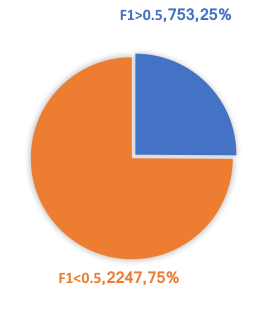
\includegraphics[width=12em]{figures/fig5.png}
%DIFDELCMD < %%%
%DIFDELCMD < \caption{%
{%DIFAUXCMD
\DIFdelFL{Prediction Results for User Based CM View Time \textperiodcentered  Purchase Intention Category 4}}
%DIFAUXCMD
%DIFDELCMD < \label{fig:5}
%DIFDELCMD < \end{figure}
%DIFDELCMD < 

%DIFDELCMD < %%%
\subsection{\DIFdel{XGBoost Comparison to SVM}}
%DIFAUXCMD
\addtocounter{subsection}{-1}%DIFAUXCMD
%DIFDELCMD < \label{svmxgboost}
%DIFDELCMD < 

%DIFDELCMD < %%%
\DIFdel{As the results shown above are all from the experiments done with SVM machine learning algorithms, we show a comparison of the experiments done with XGboost in Table \ref{tab:svmxgboost_product} and Table \ref{tab:svmxgboos_user}, for product based models and user based models respectively. 
}%DIFDELCMD < 

\DIFdel{The results for SVM prediction models held a slightly higher percentage of predictable elements, but overall they both show similar results. 
}%DIFDELCMD < 


\section{Discussion}
\label{discussion}
\DIFaddend 

\subsection{Influence of TV adverts on Actual Purchase and Purchase Intention}
\label{disc_ap_pi}

\DIFdel{In this paper, we have obtained results on the predictability of Actual Purchase and Purchase Intention customer behaviors }\DIFdelend \DIFaddbegin \DIFadd{Observing our results across models in the Tables of section \ref{av_res}, in general, we can observe that SVM models perform relatively better than XGBoost models and Logistic Models, and that the differences and directional change in averages between Advert Viewing Time based models, Demographics based models, and Advert Viewing Time and Demographics based models stay consistent across SVM, XGBoost and Logistic Regression models. That is to say, low predictability in Advert Viewing Time based models compared to Demographic data models stays constant regardless of the changes in performance accross prediction techniques.}\DIFaddend 

\DIFaddbegin \DIFadd{In Tables \ref{tab:svm_product_av_res} and \ref{tab:svm_user_av_res} we can observe this more closely. In general for Actual Purchase behavior, predictions using Advert Viewing Time only have a lower performance than the other models. Specially in categories 2 and 4 of the purchase behavior, we can see that the average predictabiity rises from 0 or close to 0, to a higher predictability in every case that demographic data is used. The exception to this rule is in category 1 of the data, where customers consistently answered "NO" in their purchase recall or purchase intention questions of the survey both in January 2017 and March 2017. Predictions seem to be high across all models, but this is irrelevant since the customer is not changing their negative purchase behavior.}\DIFaddend

\DIFaddbegin \DIFadd{We can confirm this increase is statistically significant by observing the results of Hypothesis \ref{hyp:1} in Table \ref{tab:h1_ap}. For the most part, excluding negative purchase behavior, the data is significantly different at a 95\% confidence level (\(p<0.05\)) between models that use advert viewing time as a base for prediction and models that use demographic data as a base for prediction. Moreover, we can confirm that the changes in predictability between models that include both advert viewing time and demographic data, and models that only include demographic data are not statistically significant by observing the results of Hypothesis \ref{hyp:2} in Table \ref{tab:h2_ap}. In most cases, (\(p>0.05\)), proving that the advert viewing time data did not influence the prediction scores significantly, and that whatever correct predictions were made were most likely }\DIFaddend based on the \DIFdelbegin \DIFdel{time spent exposed to TV adverts. These results would not only be useful in predicting the purchasing behavior of customers, but it would be useful as a direct measure of the effectiveness of mere exposure to advertisements. 
However, these results are low enough that it can be said }\DIFdelend \DIFaddbegin \DIFadd{coefficients and weights of the demographic data. Finally, observing Hypothesis \ref{hyp:3} in Table \ref{tab:h3_ap} also confirms the difference and increase of performance between advert viewing time models and those that combine advert data with demographic data. 
}

\DIFadd{With these results in mind, it could be said that }\DIFaddend TV adverts are not a main factor in predicting whether a customer will change their purchasing behavior \DIFaddbegin \DIFadd{or not, specially their actual purchase behavior}\DIFaddend . While the research based on the mere exposure effect would suggest otherwise, customers are observed to decide on their purchase without much predictability\DIFaddbegin \DIFadd{, except for their demographic data}\DIFaddend . It could be said that while there \DIFdelbegin \DIFdel{is }\DIFdelend \DIFaddbegin \DIFadd{might be }\DIFaddend influence in the customer's knowledge of the brand, the \DIFaddbegin \DIFadd{data suggests that the }\DIFaddend amount of time exposed to TV adverts \DIFdelbegin \DIFdel{seems to have an indirect influence on purchasing behaviorat most, if not none at all}\DIFdelend \DIFaddbegin \DIFadd{has no effect in the customers Actual Purchase behavior}\DIFaddend .

Other studies, using a controlled environment, have linked mere exposure with bias in consumer choice \cite{janiszewski}. However, there is a possible explanation for these discrepancies in results. While controlled experiments show the TV adverts to their sample audience directly in most cases, in an uncontrolled environment of a customer's home, the customer is left free to ignore the advert and do something unrelated in the meanwhile \cite{abernethy}. In the United Kingdom, there is a widely documented phenomenon involving TV advert timing and a surge in electricity caused by the use of electric kettles for preparing tea. This phenomenon is commonly called TV pickup, and has been documented for long \cite{bunn,boait}. Similar to these cases, if the customers whose data were actively ignoring the adverts, the sample for training the prediction models would contain noise, altering the results. It stands to reason that without the influence of this active aversion would have on our learning model, it might correctly predict purchasing behavior as expected. However, this is more of a problem with the current TV advertisement model than with the methodology of this study. We will discuss this further in section \ref{disc_advert} of this paper.


\subsection{Influence of TV adverts based on Primetime}
\label{disc_prime}

In our prediction model experiments, we used data from advertisement exposure during different time periods, days of the week and weekends. While we did this in order to observe differences in predictability for different time schedules available to different kinds of customers, especially during primetime television hours, we arrived to \DIFdelbegin \DIFdel{similarly low }\DIFdelend \DIFaddbegin \DIFadd{similar }\DIFaddend results for all time \DIFdelbegin \DIFdel{categories}\DIFdelend \DIFaddbegin \DIFadd{data configurations}\DIFaddend . We did not observe any difference in predictability based on Primetime television watching compared to other time periods\DIFdelbegin \DIFdel{, as well as differences in weekdays and weekends}\DIFdelend . This could be interpreted as there being little influence in time periods and changes in purchasing behavior. 
\DIFdelbegin \DIFdel{However, as we stated in section \ref{disc_ap_pi}, the common problem with advertisements being actively ignored by customers has existed for long. Taking this problem into consideration, our results imply that the problem is constant over all the time periods, and that there is not a particular time slot that results in customers being more attentive to adverts.
}\DIFdelend 

\subsection{Implications for the TV advert industry}
\label{disc_advert}

Based on the low results of predictability of purchase behavior by advert exposure, it can be observed that TV adverts have a low probability of achieving their main purpose: to increase sales. As was stated in section \ref{disc_ap_pi} of this paper, there could be a large influence on this study's results from customers actively ignoring the adverts although they are being broadcast to their TVs. It is left to further discussion and research if adverts actually have the intended effect on customers when watched properly, or if this effect is not achieved anyway. In \cite{fang} it is proposed that while the mere exposure of banner advertisement increases perceptual fluency, it doesn't have an effect on actual brand recognition compared to the control groups, for example. The existence or absence of influence by perceptual fluency on a customer's purchase decision hasn't been fully explored, but the consensus in the processing fluency model is that perceptual fluency influences brand judgement on some level, although it depends on the concept if the reception is positive or not \cite{lee-a}. The problem with these studies and the current consensus, as has been said previously in this paper, is both that most experiments are done with relatively small sample sizes, and that there is a factor of uncertainty that comes with the physical avoidance of adverts in a \DIFdelbegin \DIFdel{customers home environment}\DIFdelend \DIFaddbegin \DIFadd{customer's household}\DIFaddend .

With these things in mind, we consider both possibilities: either customers are attentive and the adverts have the expected influence in their short and long term memories in the case of repeated exposures \cite{rossiter}; or the customers are inattentive of the advert and there might be some level of unconscious effect of mere exposure in their perception fluency \cite{fang}. We observed however in our results that \DIFdelbegin \DIFdel{the }\DIFdelend \DIFaddbegin \DIFadd{there is no }\DIFaddend effect on Actual Purchase behavior\DIFdelbegin \DIFdel{is minimal}\DIFdelend . While it may be true and out of the reach of our data that the customers would have influence in their memory, there was no link observed between the time of advert exposure and the purchase decisions. This raises a concern for the TV advert industry. Regardless of the cause of our results, the main implication of our paper is that currently, TV adverts are shown to have little to no effect on changes in Actual Purchase behavior\DIFdelbegin \DIFdel{, and only some observable effect in Purchase Intention}\DIFdelend . While thousands of billions of japanese yen are spent on TV advertisements each year \footnote{\label{dentsu}Dentsu, inc. 2017 Advertising Expenditures in Japan. Retrieved on May 2018 from \href {http://www.dentsu.com/knowledgeanddata/ad_expenditures/pdf/expenditures_2017.pdf}{\path{http://www.dentsu.com/knowledgeanddata/ad_expenditures/pdf/expenditures_2017.pdf}}}, the effects observed in this study are negligible. Because of this, changes are necessary in the current TV advertisement model.

\DIFaddbegin \section{\DIFadd{Limitations}}
\label{limitations}

\DIFadd{In comparison with previous research regarding this topic, our study presents a much larger database, a sample of 3000 users for 36 different products and the previously unavailable household television viewing data increases the possibilities for studying the effects of advert exposure more realistically. In accordance to this size of data, we used SVM and XGBoost, which are considered well performing machine learning algorithms in this level of magnitude. However, while we propose using machine learning algorithms as an effective method, we are still limited by the magnitude of the data. Top performing and state of the art models, such as Deep Neural Networks, with their variations and advancements, use datasents with orders of magnitude much larger (for example, 3,000,000 users instead of 3,000, and thousands more products instead of 36) in order to perform to the level that they are praised for. The calculation time also increases greatly, and is more appropriate for single models being trained, instead of a comparison of a large array of models. 
}

\DIFadd{Another limitation of this study is the nature of the prediction targets collected by survey. While a person can be asked directly in a survey whether they would purchase an item (purchase intention) or if they had already in the recent past (actual purchase), research based on online shopping has access to the actual purchase data, and to the number of times a person looks at a products description page, or searches terms related to it. Television advertisement research, by its nature, is harder to connect to the actual behavior of the customers and can only be assumed to be equal to their reported behavior. There is also a limitation of the number of questions that a person might answer, and how honestly they might answer them with a survey of this magnitude.
}

\DIFadd{In addition to this, because of the timing of the surveys being 3 months appart between January and March 2017, we can only examine the short-term effect of advertisements, and not the long-term effect across different years of constant advertisement exposure.
}

\DIFadd{Furthermore, much of the data that could be used to inspect this matter further belongs to private institutions and in many cases, is treated as a company secret. 
}

\DIFadd{However, with the measurements of short-term effects of advertisement in a field where not much new research is done, we can start to shed light on problems that could be having a large impact on the costs of many industries.
}

\DIFaddend \section{Conclusion and Future Work}
\label{conclusion}

In this paper we analyzed the ability to predict purchasing behavior, namely \DIFdelbegin \DIFdel{Purchase Intention and }\DIFdelend Actual Purchase \DIFaddbegin \DIFadd{and Purchase Intention, }\DIFaddend based on the customers' time spent exposed to television adverts using machine learning algorithms\DIFdelbegin \DIFdel{. We analyzed the data by product and by customer, determining which specific products and which specific customers provided a better prediction model}\DIFdelend \DIFaddbegin \DIFadd{, and compared it to the ability to predict the same behavior by using demographic data on its own and in combination with the exposure time data}\DIFaddend . Based on \DIFdelbegin \DIFdel{our low results for any prediction }\DIFdelend \DIFaddbegin \DIFadd{the low prediction results }\DIFaddend of Actual Purchase \DIFdelbegin \DIFdel{, we concluded that there must be other factors that are more strongly tied to the customer's purchasing behavior. The results for Purchase Intention were relatively higher but still low enough that only a few products, mostly tea and chocolate snacks, could be predicted, and only one fourth of the customers were predictable in their purchase intention. 
}\DIFdelend \DIFaddbegin \DIFadd{by exposure time models and the relatively high prediction results for demographic based models, as well as a non-significant difference between the demographic models and the combined models, we concluded that advertisement exposure has little to no effect in short-time Actual Purchase behavior. 
}

\DIFaddend We discussed possible influence by deliberate avoidance of advert cuts to prepare food or tea, and while some studies focus on the effect of attentive watching of adverts, other studies focus on the mere exposure effects, which would be achieved despite physical avoidance because of advert audio and simple proximity of the television. Both scenarios are in strong contrast with the results of our study, which shows little to no predictability in purchase behavior. Points left to research in future work are a deeper analysis of the predictable customers, looking for similarities or clusters within this class, as well as using \DIFdelbegin \DIFdel{different machine learning algorithms , which weren't considered because of requiring bigger datasets }\DIFdelend \DIFaddbegin \DIFadd{newer and better performing deep learning algorithms when larger datasets are available}\DIFaddend . 

\section{Acknowledgements}

This paper was made possible by the data provided by Nomura Research Institute, Ltd. for their yearly Marketing Analysis Contest.

Declarations of interest: none

\section*{References}

\bibliography{ipmbibfile}

%DIF <  \usepackage{filecontents}
%DIF <  \begin{filecontents}{\ipmbibfile.bib}
%DIF <  @article{1,
%DIF <  author = {Armstrong, J. and Morwitz, V. and Kumar, V.},
%DIF <  journal = {International Journal Of Forecasting},
%DIF <  number = {3},
%DIF <  pages = {383-397},
%DIF <  title = {Sales forecasts for existing consumer products and services: Do purchase intentions contribute to accuracy?},
%DIF <  volume = {16},
%DIF <  year = {2000},
%DIF <  doi = {10.1016/s0169-2070(00)00058-3},
%DIF <  }
\DIFaddbegin \clearpage
\appendix
\appendixpage
\DIFaddend 

%DIF <  @article{2,
%DIF <  author = {Morwitz, V. and Steckel, J. and Gupta, A.},
%DIF <  journal = {International Journal Of Forecasting},
%DIF <  number = {3},
%DIF <  pages = {347-364},
%DIF <  title = {When do purchase intentions predict sales?},
%DIF <  volume = {23},
%DIF <  year = {2007},
%DIF <  doi = {10.1016/j.ijforecast.2007.05.015},
%DIF <  }
\DIFaddbegin \section{\DIFadd{Input Data Details}}
\label{appendix:inputs}
\DIFaddend 

%DIF <  @article{3,
%DIF <  author = {Khuong, M. and Nguyen, T.},
%DIF <  journal = {Journal Of Economics, Business And Management},
%DIF <  number = {9},
%DIF <  pages = {851-857},
%DIF <  title = {The Effects of Television Commercials on Customers Purchase Intention -- A Study of Milk Industry in Ho Chi Minh City, Vietnam},
%DIF <  volume = {3},
%DIF <  year = {2015},
%DIF <  }
\DIFaddbegin \DIFadd{As explained in section \ref{advert_viewtime}, two data configurations were used for advert viewing time. The detailed features used are shown in Table \ref{tab:viewtimes}. 
}\DIFaddend 

%DIF <  @article{4,
%DIF <  author = {Sun, B. and Morwitz, V.},
%DIF <  journal = {International Journal Of Research In Marketing},
%DIF <  number = {4},
%DIF <  pages = {356-366},
%DIF <  title = {Stated intentions and purchase behavior: A unified model},
%DIF <  volume = {27},
%DIF <  year = {2010},
%DIF <  doi = {10.1016/j.ijresmar.2010.06.001},
%DIF <  }
\DIFaddbegin \DIFadd{Similarly, as explained in section \ref{demographics}, demographic data was used as input for predictions in a number of our experiments. The detailed features used in the input vectors are described in Table \ref{tab:demographics}.
}\DIFaddend 

%DIF <  @article{5,
%DIF <  author = {Newberry, C. and Klemz, B. and Boshoff, C.},
%DIF <  journal = {Journal Of Services Marketing},
%DIF <  number = {6},
%DIF <  pages = {609-620},
%DIF <  title = {Managerial implications of predicting purchase behavior from purchase intentions: a retail patronage case study},
%DIF <  volume = {17},
%DIF <  year = {2003},
%DIF <  doi = {10.1108/08876040310495636},
%DIF <  }
\DIFaddbegin \begin{table}[htp] \centering
\caption{\DIFaddFL{Viewing time analysis elements}}\label{tab:viewtimes}
\rowcolors{2}{DarkLime}{LightGreen}
\begin{tabular}{|m{11em}|l|}  \arrayrulecolor{white} \hline
\rowcolor{DeepGreen}
\color{white}\textbf{\DIFaddFL{Data Configuration}} & \color{white}\textbf{\begin{tabular}[c]{@{}l@{}}\DIFaddFL{Advert Viewing Time in seconds }\\ \DIFaddFL{Data Features }\end{tabular}} \\ \hline
\textbf{\DIFaddFL{Weekdays}}           
    & \begin{tabular}[c]{@{}l@{}}
    \DIFaddFL{$\bullet$ Monday}\\ 
    \DIFaddFL{$\bullet$ Tuesday}\\ 
    \DIFaddFL{$\bullet$ Wednesday}\\ 
    \DIFaddFL{$\bullet$ Thursday}\\ 
    \DIFaddFL{$\bullet$ Friday}\\ 
    \DIFaddFL{$\bullet$ Saturday}\\ 
    \DIFaddFL{$\bullet$ Sunday}\end{tabular} \\ \hline
\textbf{\DIFaddFL{Weekday Time Slots}} 
    & \begin{tabular}[c]{@{}l@{}}
    \DIFaddFL{$\bullet$ Monday Primetime}\\ 
    \DIFaddFL{$\bullet$ Monday Non-Primetime}\\ 
    \DIFaddFL{$\bullet$ Tuesday Primetime}\\ 
    \DIFaddFL{$\bullet$ Tuesday Non-Primetime}\\ 
    \DIFaddFL{$\bullet$ Wednesday Primetime}\\ 
    \DIFaddFL{$\bullet$ Wednesday Non-Primetime}\\ 
    \DIFaddFL{$\bullet$ Thursday Primetime}\\ 
    \DIFaddFL{$\bullet$ Thursday Non-Primetime}\\ 
    \DIFaddFL{$\bullet$ Friday Primetime}\\ 
    \DIFaddFL{$\bullet$ Friday Non-Primetime}\\ 
    \DIFaddFL{$\bullet$ Saturday Primetime}\\ 
    \DIFaddFL{$\bullet$ Saturday Non-Primetime}\\ 
    \DIFaddFL{$\bullet$ Sunday Primetime}\\ 
    \DIFaddFL{$\bullet$ Sunday Non-Primetime }\end{tabular} \\ \hline
\end{tabular}
\end{table}
\DIFaddend 



%DIF <  @article{6,
%DIF <  author = {Shareef, M. and Mukerji, B. and Alryalat, M. and Wright, A. and Dwivedi, Y.},
%DIF <  journal = {Journal Of Retailing And Consumer Services},
%DIF <  pages = {258-268},
%DIF <  title = {Advertisements on Facebook: Identifying the persuasive elements in the development of positive attitudes in consumers},
%DIF <  volume = {43},
%DIF <  year = {2018},
%DIF <  doi = {10.1016/j.jretconser.2018.04.006},
%DIF <  }
\DIFaddbegin \begin{table}[htp] \centering
\caption{\DIFaddFL{Demographic data used in input vectors}}\label{tab:demographics}
\rowcolors{2}{DarkLiliac}{Liliac}
\begin{tabular}{|l|l|} \arrayrulecolor{white} \hline
\rowcolor{DeepPurple}
\color{white}\textbf{\DIFaddFL{Survey Data}}     & \color{white}\textbf{\DIFaddFL{Possible Answers}} \\ \hline
\textbf{\DIFaddFL{Age}}
    & \begin{tabular}[c]{@{}l@{}}
    \DIFaddFL{$\bullet$ 18 to 25 years old}\\ 
    \DIFaddFL{$\bullet$ 26 to 35 years old}\\ 
    \DIFaddFL{$\bullet$ 36 to 45 years old}\\ 
    \DIFaddFL{$\bullet$ 46 to 55 years old}\\ 
    \DIFaddFL{$\bullet$ 56 or older}\end{tabular} \\ \hline
\textbf{\DIFaddFL{Sex}}
    & \begin{tabular}[c]{@{}l@{}}
    \DIFaddFL{$\bullet$ Male}\\ 
    \DIFaddFL{$\bullet$ Female}\end{tabular} \\ \hline
\textbf{\DIFaddFL{Marital Status}}
    & \begin{tabular}[c]{@{}l@{}}
    \DIFaddFL{$\bullet$ Single}\\ 
    \DIFaddFL{$\bullet$ Married}\\ 
    \DIFaddFL{$\bullet$ Divorced or Widowed}\end{tabular} \\ \hline
\textbf{\DIFaddFL{Parental Status}}
    & \begin{tabular}[c]{@{}l@{}}
    \DIFaddFL{$\bullet$ Parent}\\ 
    \DIFaddFL{$\bullet$ Not a Parent}\end{tabular} \\ \hline
\textbf{\DIFaddFL{Income Bracket}}
    & \begin{tabular}[c]{@{}l@{}}
    \DIFaddFL{$\bullet$ Not disclosed}\\ 
    \DIFaddFL{$\bullet$ No Income}\\ 
    \DIFaddFL{$\bullet$ Under 1,000,000 yen}\\ 
    \DIFaddFL{$\bullet$ From 1,000,000 yen to 2,000,000 yen}\\ 
    \DIFaddFL{$\bullet$ From 2,000,000 yen to 3,000,000 yen}\\ 
    \DIFaddFL{$\bullet$ From 3,000,000 yen to 4,000,000 yen}\\ 
    \DIFaddFL{$\bullet$ From 4,000,000 yen to 5,000,000 yen}\\ 
    \DIFaddFL{$\bullet$ From 5,000,000 yen to 6,000,000 yen}\\ 
    \DIFaddFL{$\bullet$ From 6,000,000 yen to 7,000,000 yen}\\ 
    \DIFaddFL{$\bullet$ From 7,000,000 yen to 10,000,000 yen}\\ 
    \DIFaddFL{$\bullet$ From 10,000,000 yen to 15,000,000 yen}\\ 
    \DIFaddFL{$\bullet$ From 15,000,000 yen to 20,000,000 yen}\\ 
    \DIFaddFL{$\bullet$ Over 20,000,000 yen}\end{tabular} \\ \hline
\end{tabular}
\end{table}
\DIFaddend 


%DIF <  @article{7,
%DIF <  author = {Gonzalez Camacho, L. and Alves-Souza, S.},
%DIF <  journal = {Information Processing \& Management},
%DIF <  number = {4},
%DIF <  pages = {529-544},
%DIF <  title = {Social network data to alleviate cold-start in recommender system: A systematic review},
%DIF <  volume = {54},
%DIF <  year = {2018},
%DIF <  doi = {10.1016/j.ipm.2018.03.004},
%DIF <  }
\DIFaddbegin \section{\DIFadd{Data Distribution}}
\label{data_dist}
\DIFaddend 

%DIF <  @article{8,
%DIF <  author = {Ramaboa, K. and Fish, P.},
%DIF <  journal = {Information Processing \& Management},
%DIF <  number = {2},
%DIF <  pages = {175-183},
%DIF <  title = {Keyword length and matching options as indicators of search intent in sponsored search},
%DIF <  volume = {54},
%DIF <  year = {2018},
%DIF <  doi = {10.1016/j.ipm.2017.11.003},
%DIF <  }
\DIFaddbegin \DIFadd{In this section we will describe the data we received from the Nomura Research Institute, Ltd., and the distribution and nature of products, adverts and prediction targets.
}\DIFaddend 

%DIF <  @article{9,
%DIF <  author = {Wu, C. and Kao, S. and Wu, C. and Huang, S.},
%DIF <  journal = {Information Processing \& Management},
%DIF <  number = {5},
%DIF <  pages = {625-642},
%DIF <  title = {Location-aware service applied to mobile short message advertising: Design, development, and evaluation},
%DIF <  volume = {51},
%DIF <  year = {2015},
%DIF <  doi = {10.1016/j.ipm.2015.06.001},
%DIF <  }
\DIFaddbegin \subsection{\DIFadd{Surveyed Products}}
\label{product_data}
\DIFaddend 

%DIF <  @article{10,
%DIF <  author = {Zajonc, R.},
%DIF <  journal = {Journal Of Personality And Social Psychology},
%DIF <  number = {2 Pt.2},
%DIF <  pages = {1-27},
%DIF <  title = {Attitudinal effects of mere exposure},
%DIF <  volume = {9},
%DIF <  year = {1968},
%DIF <  doi = {10.1037/h0025848},
%DIF <  }
\DIFaddbegin \DIFadd{The surveys of purchase behavior taken in January 2017 and March 2017 included 200 products, from which only 36 were matched to television adverts during the period between both surveys. Because most of the products are sold only in Japan, a general description of their nature and distribution is explained in Figure \ref{fig:product_dist}. 
}\DIFaddend 

%DIF <  @article{11,
%DIF <  author = {Hekkert, P. and Thurgood, C. and Whitfield, T.},
%DIF <  journal = {Acta Psychologica},
%DIF <  number = {2},
%DIF <  pages = {411-417},
%DIF <  title = {The mere exposure effect for consumer products as a consequence of existing familiarity and controlled exposure},
%DIF <  volume = {144},
%DIF <  year = {2013},
%DIF <  doi = {10.1016/j.actpsy.2013.07.015},
%DIF <  }
%DIF >  The general distribution of products in the entire survey is shown in Figure \ref{fig:product_dist_200}

%DIF <  @article{12,
%DIF <  author = {Huang, Y. and Hsieh, P.},
%DIF <  journal = {Vision Research},
%DIF <  pages = {56-61},
%DIF <  title = {The mere exposure effect is modulated by selective attention but not visual awareness},
%DIF <  volume = {91},
%DIF <  year = {2013},
%DIF <  doi = {10.1016/j.visres.2013.07.017},
%DIF <  }
\DIFaddbegin \begin{figure}[htp]
\centering
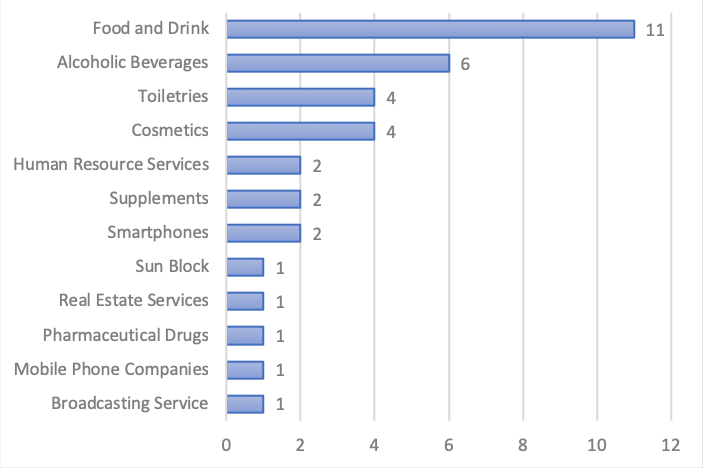
\includegraphics[width=35em]{figures/product_categories_36.png}
\caption{\DIFaddFL{Products Matched with Advert Viewing Data}}
\label{fig:product_dist}
\end{figure} 
\DIFaddend 

%DIF <  @article{13,
%DIF <  author = {Dech{\^e}ne, A. and Stahl, C. and Hansen, J. and W{"a}nke, M.},
%DIF <  journal = {Journal Of Experimental Social Psychology},
%DIF <  number = {5},
%DIF <  pages = {1117-1122},
%DIF <  title = {Mix me a list: Context moderates the truth effect and the mere-exposure effect},
%DIF <  volume = {45},
%DIF <  year = {2009},
%DIF <  doi = {10.1016/j.jesp.2009.06.019},
%DIF <  }
%DIF >  \begin{figure}
%DIF >  \centering
%DIF >  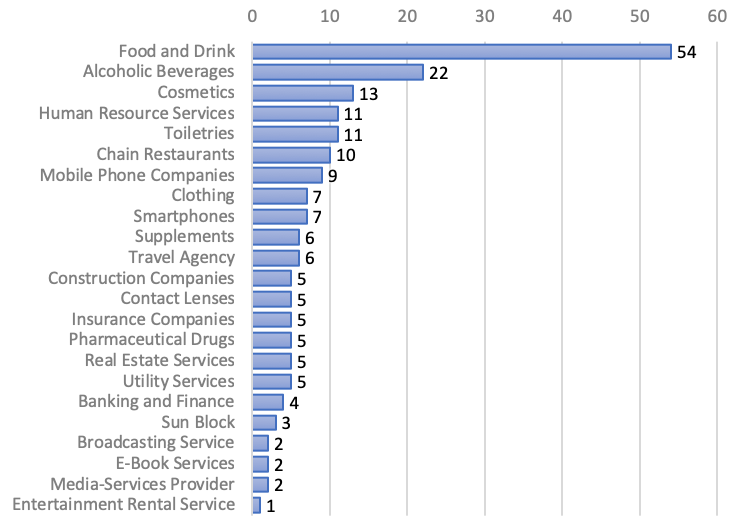
\includegraphics{figures/product_categories_200.png}
%DIF >  \caption{Products in Survey Data}
%DIF >  \label{fig:product_dist_200}
%DIF >  \end{figure} 

%DIF <  @article{14,
%DIF <  author = {Fang, X. and Singh, S. and Ahluwalia, R.},
%DIF <  journal = {Journal Of Consumer Research},
%DIF <  number = {1},
%DIF <  pages = {97-103},
%DIF <  title = {An Examination of Different Explanations for the Mere Exposure Effect},
%DIF <  volume = {34},
%DIF <  year = {2007},
%DIF <  doi = {10.1086/513050},
%DIF <  }
\DIFaddbegin \subsection{\DIFadd{Advert Exposure and Broadcasting Data}}
\label{advert_broadcast_dist}
\DIFaddend 

%DIF <  @article{15,
%DIF <  author = {Gmuer, A. and Siegrist, M. and Dohle, S.},
%DIF <  journal = {Food Quality And Preference},
%DIF <  pages = {12-16},
%DIF <  title = {Does wine label processing fluency influence wine hedonics?},
%DIF <  volume = {44},
%DIF <  year = {2015},
%DIF <  doi = {10.1016/j.foodqual.2015.03.007},
%DIF <  }
\DIFaddbegin \DIFadd{The data we received from the Nomura Research Institute, Ltd. included the surveyees' household television viewing times and the program that was displayed when television was on. By matching this data with the adverts that were in between breaks from those programs for the products that were surveyed, we obtained the advert exposure time for each user for each product. In this study we explore the possibility of there being some difference in effect depending on the time slot, particularly the Primetime (19:00 to 23:00) time slot. In Figure \ref{fig:broadcast_dist} we show the broadcasting time distribution for the programs that displayed these 36 products during the period of time in between the survey in January 2017 and the survey in March 2017. In Figure \ref{fig:exposure_dist} we show the total sum of exposure time in seconds across all users and products for the Primetime and otherwise time slots for each day of the week.
}\DIFaddend 


%DIF <  @article{16,
%DIF <  author = {Schwarz, N.},
%DIF <  journal = {Journal Of Consumer Psychology},
%DIF <  number = {4},
%DIF <  pages = {332-348},
%DIF <  title = {Metacognitive Experiences in Consumer Judgment and Decision Making},
%DIF <  volume = {14},
%DIF <  year = {2004},
%DIF <  doi = {10.1207/s15327663jcp1404_2},
%DIF <  }
\DIFaddbegin \begin{figure}[htp]
\centering
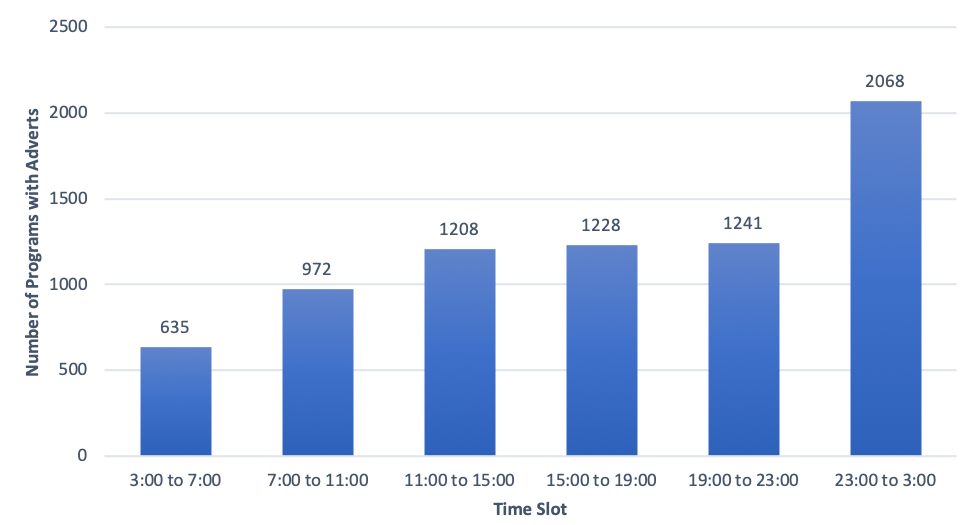
\includegraphics[width=35em]{figures/broadcast_distributions.png}
\caption{\DIFaddFL{Programs including adverts broadcast time distribution}}
\label{fig:broadcast_dist}
\end{figure} 
\DIFaddend 

%DIF <  @article{17,
%DIF <  author = {Silva, R. and Garcia-Marques, T. and Reber, R.},
%DIF <  journal = {Consciousness And Cognition},
%DIF <  pages = {53-67},
%DIF <  title = {The informative value of type of repetition: Perceptual and conceptual fluency influences on judgments of truth},
%DIF <  volume = {51},
%DIF <  year = {2017},
%DIF <  doi = {10.1016/j.concog.2017.02.016},
%DIF <  }
\DIFaddbegin \begin{figure}[htp]
\centering
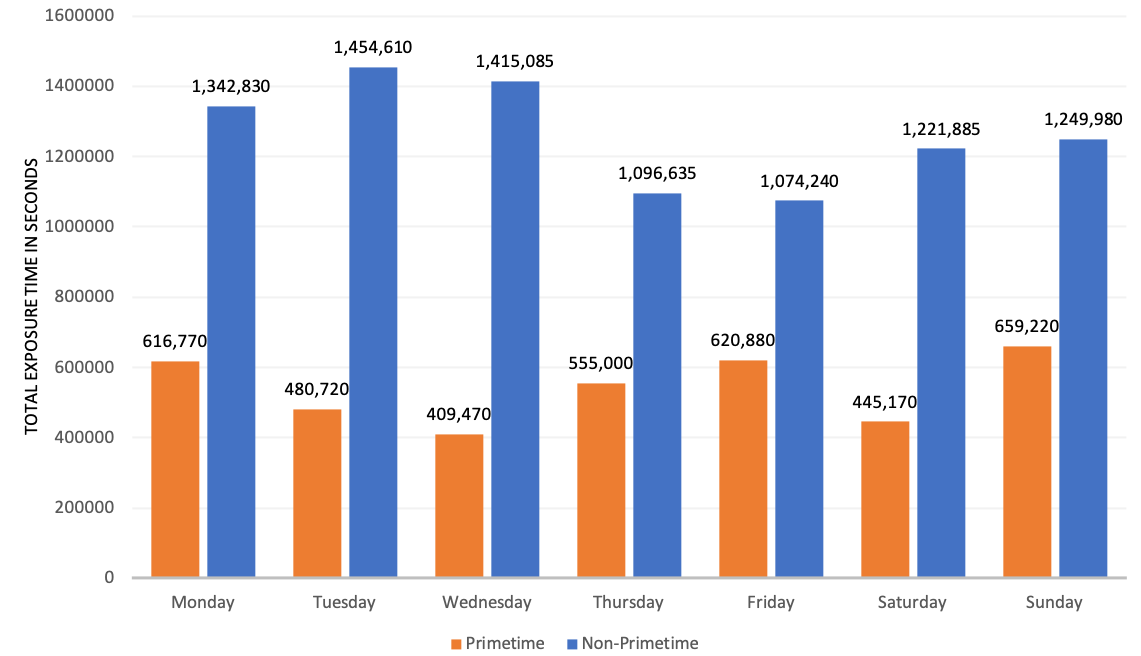
\includegraphics[width=35em]{figures/exposure_dist.png}
\caption{\DIFaddFL{Advert Exposure Time for all users and products by Weekday and Time Slot}}
\label{fig:exposure_dist}
\end{figure} 
\DIFaddend 

%DIF <  @article{18,
%DIF <  author = {Jacoby, L. and Dallas, M.},
%DIF <  journal = {Journal Of Experimental Psychology: General},
%DIF <  pages = {306-304},
%DIF <  title = {On the Relationship Between Autobiographical Memory and Perceptual Learning},
%DIF <  volume = {110},
%DIF <  year = {1981},
%DIF <  }
\DIFaddbegin \subsection{\DIFadd{Prediction Target Categories}}
\label{cat_dist}
\DIFaddend 

%DIF <  @article{19,
%DIF <  author = {Reber, R. and Winkielman, P. and Schwarz, N.},
%DIF <  journal = {Psychological Science},
%DIF <  number = {1},
%DIF <  pages = {45-48},
%DIF <  title = {Effects of Perceptual Fluency on Affective Judgments},
%DIF <  volume = {9},
%DIF <  year = {1998},
%DIF <  doi = {10.1111/1467-9280.00008},
%DIF <  }
\DIFaddbegin \DIFadd{The surveys included data of purchase intention and actual purchase at the times of January 2017 and March 2017 for 200 products, 36 of which were matched with television advert viewing data. As was explained in section \ref{target_data_cat} and in Tables \ref{tab:categories_ap} and \ref{tab:categories_pi}, we divided the data in 6 categories (0 to 5) in order to observe the changes in time for these purchase behaviors. The distributions of these categories are shown in Table \ref{tab:cat_dist}. Note that categories 4 and 5, by their nature, are a sum of categories 2 and 3, and 0 and 1 respectively. 
}\DIFaddend 

%DIF <  @article{20,
%DIF <  author = {Seamon, J. and Williams, P. and Crowley, M. and Kim, I. and Langer, S. and Orne, P. and Wishengrad, D.},
%DIF <  journal = {Journal Of Experimental Psychology: Learning, Memory And Cognition},
%DIF <  number = {3},
%DIF <  pages = {711-721},
%DIF <  title = {The Mere Exposure Effect Is Based On Implicit Memory: Effects of Stimulus Type, Encoding Conditions, and Number of Exposures on Recognition and Affect Judgements},
%DIF <  volume = {21},
%DIF <  year = {1995},
%DIF <  }
\DIFaddbegin \begin{table}[p] \centering
\caption{\DIFaddFL{Prediction Target Categories Distribution}}\label{tab:cat_dist}
\begin{tabular}{|>{\columncolor{SweetPlum}}=c|>{\columncolor{Salmon}}+r|>{\columncolor{Liliac}}+r|>{\columncolor{Salmon}}+r|>{\columncolor{Liliac}}+r|} \arrayrulecolor{white} \hline
\rowcolor{Plum}
\DIFaddendFL 

%DIF <  @article{21,
%DIF <  author = {Lee, A. and Labroo, A.},
%DIF <  journal = {Journal Of Marketing Research},
%DIF <  number = {2},
%DIF <  pages = {151-165},
%DIF <  title = {The Effect of Conceptual and Perceptual Fluency on Brand Evaluation},
%DIF <  volume = {41},
%DIF <  year = {2004},
%DIF <  doi = {10.1509/jmkr.41.2.151.28665},
%DIF <  }
\DIFaddbeginFL \cellcolor{white}{}    & \multicolumn{2}{c|}{\color{white}\textbf{All products (200)}} & \multicolumn{2}{c|}{\begin{tabular}[c]{@{}c@{}}\color{white}\textbf{Advert matched} \\ \color{white}\textbf{products (36)}\end{tabular}} \\ \hline
\rowstyle{\bfseries}
\cellcolor{Plum}\color{white}\DIFaddFL{Category
    }& \cellcolor{DarkSalmon}\begin{tabular}[c]{@{}c@{}}\DIFaddFL{Actual }\\ \DIFaddFL{Purchase }\end{tabular} 
    & \cellcolor{DarkLiliac}\begin{tabular}[c]{@{}c@{}}\DIFaddFL{Purchase }\\ \DIFaddFL{Intention }\end{tabular} 
    & \cellcolor{DarkSalmon}\begin{tabular}[c]{@{}c@{}}\DIFaddFL{Actual }\\ \DIFaddFL{Purchase }\end{tabular}
    & \cellcolor{DarkLiliac}\begin{tabular}[c]{@{}c@{}}\DIFaddFL{Purchase }\\ \DIFaddFL{Intention }\end{tabular} \\ \hline
\DIFaddendFL 

    %DIF <  @article{22,
%DIF <  author = {Boyland, E. and Halford, J.},
%DIF <  journal = {Appetite},
%DIF <  pages = {236-241},
%DIF <  title = {Television advertising and branding: Effects on eating behaviour and food preferences in children},
%DIF <  volume = {62},
%DIF <  year = {2013},
%DIF <  doi = {10.1016/j.appet.2012.01.032},
%DIF <  }
\DIFdelbeginFL %DIFDELCMD < 

%DIFDELCMD < %%%
%DIF <  @article{23,
%DIF <  author = {Rossiter, J. and Silberstein, R. and Harris, P. and Nield, G.},
%DIF <  journal = {Journal Of Advertising Research},
%DIF <  number = {2},
%DIF <  pages = {13-21},
%DIF <  title = {Brain-Imaging Detection of Visual Scene Encoding in Long-term Memory for TV Commercials},
%DIF <  volume = {41},
%DIF <  year = {2001},
%DIF <  doi = {10.2501/jar-41-2-13-21},
%DIF <  }
%DIFDELCMD < 

%DIFDELCMD < %%%
%DIF <  @inproceedings{24,
%DIF <  address = {San Diego, California, USA},
%DIF <  author = {Stitelman, O. and Dalessandro, B. and Perlich, C. and Provost, F.},
%DIF <  booktitle = {Proceedings of the Fifth International Workshop on Data Mining and Audience Intelligence for Advertising (ADKDD 2011)},
%DIF <  title = {Estimating the effect of online display advertising on browser conversion},
%DIF <  year = {2011},
%DIF <  pages = {8-16}
%DIF <  }
%DIFDELCMD < 

%DIFDELCMD < %%%
%DIF <  @article{25,
%DIF <  author = {Perlich, C. and Dalessandro, B. and Raeder, T. and Stitelman, O. and Provost, F.},
%DIF <  journal = {Machine Learning},
%DIF <  number = {1},
%DIF <  pages = {103-127},
%DIF <  title = {Machine learning for targeted display advertising: transfer learning in action},
%DIF <  volume = {95},
%DIF <  year = {2013},
%DIF <  doi = {10.1007/s10994-013-5375-2},
%DIF <  }
%DIFDELCMD < 

%DIFDELCMD < %%%
%DIF <  @article{26,
%DIF <  author = {Schwartz, E. and Bradlow, E. and Fader, P.},
%DIF <  journal = {Marketing Science},
%DIF <  number = {4},
%DIF <  pages = {500-522},
%DIF <  title = {Customer Acquisition via Display Advertising Using Multi-Armed Bandit Experiments},
%DIF <  volume = {36},
%DIF <  year = {2017},
%DIF <  doi = {10.1287/mksc.2016.1023},
%DIF <  }
%DIFDELCMD < 

%DIFDELCMD < %%%
%DIF <  @article{27,
%DIF <  author = {Shareef, M. and Mukerji, B. and Dwivedi, Y. and Rana, N. and Islam, R.},
%DIF <  journal = {Journal Of Retailing And Consumer Services},
%DIF <  title = {Social media marketing: Comparative effect of advertisement sources},
%DIF <  year = {2017},
%DIF <  doi = {10.1016/j.jretconser.2017.11.001},
%DIF <  }
%DIFDELCMD < 

%DIFDELCMD < %%%
%DIF <  @article{28,
%DIF <  author = {Jansen, B. and Moore, K. and Carman, S.},
%DIF <  journal = {Information Processing \& Management},
%DIF <  number = {1},
%DIF <  pages = {286-302},
%DIF <  title = {Evaluating the performance of demographic targeting using gender in sponsored search},
%DIF <  volume = {49},
%DIF <  year = {2013},
%DIF <  doi = {10.1016/j.ipm.2012.06.001},
%DIF <  }
%DIFDELCMD < 

%DIFDELCMD < %%%
%DIF <  @article{29,
%DIF <  author = {Zhang, Y. and Zhang, W. and Gao, B. and Yuan, X. and Liu, T.},
%DIF <  journal = {Information Processing \& Management},
%DIF <  number = {4},
%DIF <  pages = {508-523},
%DIF <  title = {Bid keyword suggestion in sponsored search based on competitiveness and relevance},
%DIF <  volume = {50},
%DIF <  year = {2014},
%DIF <  doi = {10.1016/j.ipm.2014.02.004},
%DIF <  }
%DIFDELCMD < 

%DIFDELCMD < %%%
%DIF <  @article{30,
%DIF <  author = {Kannan, R. and Ghinea, G. and Swaminathan, S.},
%DIF <  journal = {Information Processing \& Management},
%DIF <  number = {3},
%DIF <  pages = {286-305},
%DIF <  title = {What do you wish to see? A summarization system for movies based on user preferences},
%DIF <  volume = {51},
%DIF <  year = {2015},
%DIF <  doi = {10.1016/j.ipm.2014.12.001},
%DIF <  }
%DIFDELCMD < 

%DIFDELCMD < %%%
%DIF <  @article{31,
%DIF <  author = {Choi, I. and Oh, M. and Kim, J. and Ryu, Y.},
%DIF <  journal = {International Journal Of Information Management},
%DIF <  number = {3},
%DIF <  pages = {397-402},
%DIF <  title = {Collaborative filtering with facial expressions for online video recommendation},
%DIF <  volume = {36},
%DIF <  year = {2016},
%DIF <  doi = {10.1016/j.ijinfomgt.2016.01.005},
%DIF <  }
%DIFDELCMD < 

%DIFDELCMD < %%%
%DIF <  @article{32,
%DIF <  author = {Alalwan, A.},
%DIF <  journal = {International Journal Of Information Management},
%DIF <  pages = {65-77},
%DIF <  title = {Investigating the impact of social media advertising features on customer purchase intention},
%DIF <  volume = {42},
%DIF <  year = {2018},
%DIF <  doi = {10.1016/j.ijinfomgt.2018.06.001},
%DIF <  }
%DIFDELCMD < 

%DIFDELCMD < %%%
%DIF <  @article{33,
%DIF <  author = {Lee, J. and Hong, I.},
%DIF <  journal = {International Journal Of Information Management},
%DIF <  number = {3},
%DIF <  pages = {360-373},
%DIF <  title = {Predicting positive user responses to social media advertising: The roles of emotional appeal, informativeness, and creativity},
%DIF <  volume = {36},
%DIF <  year = {2016},
%DIF <  doi = {10.1016/j.ijinfomgt.2016.01.001},
%DIF <  }
%DIFDELCMD < 

%DIFDELCMD < %%%
%DIF <  @article{34,
%DIF <  author = {Shareef, M. and Dwivedi, Y. and Kumar, V. and Kumar, U.},
%DIF <  journal = {International Journal Of Information Management},
%DIF <  number = {4},
%DIF <  pages = {257-268},
%DIF <  title = {Content design of advertisement for consumer exposure: Mobile marketing through short messaging service},
%DIF <  volume = {37},
%DIF <  year = {2017},
%DIF <  doi = {10.1016/j.ijinfomgt.2017.02.003},
%DIF <  }
%DIFDELCMD < 

%DIFDELCMD < %%%
%DIF <  @article{35,
%DIF <  author = {Cortes, C. and Vapnik, V.},
%DIF <  journal = {Machine Learning},
%DIF <  number = {3},
%DIF <  pages = {273-297},
%DIF <  title = {Support-vector networks},
%DIF <  volume = {20},
%DIF <  year = {1995},
%DIF <  doi = {10.1007/bf00994018},
%DIF <  }
%DIFDELCMD < 

%DIFDELCMD < %%%
%DIF <  @inproceedings{36,
%DIF <  address = {San Francisco, California, USA},
%DIF <  author = {Chen, T. and Guestrin, C.},
%DIF <  booktitle = {Proceedings of the 22nd ACM SIGKDD International Conference on Knowledge Discovery and Data Mining (KDD'16)},
%DIF <  pages = {785-794},
%DIF <  title = {XGBoost: A scalable tree boosting system},
%DIF <  year = {2016},
%DIF <  doi = {10.1145/2939672.2939785}
%DIF <  }
%DIFDELCMD < 

%DIFDELCMD < %%%
%DIF <  @article{37,
%DIF <  author = {Janiszewski, C.},
%DIF <  journal = {Journal Of Consumer Research},
%DIF <  number = {3},
%DIF <  pages = {376-392},
%DIF <  title = {Preattentive Mere Exposure Effects},
%DIF <  volume = {20},
%DIF <  year = {1993},
%DIF <  url = {http://www.jstor.org/stable/2489354},
%DIF <  }
%DIFDELCMD < 

%DIFDELCMD < %%%
%DIF <  @article{38,
%DIF <  author = {Abernethy, A.},
%DIF <  journal = {Current Issues And Research In Advertising},
%DIF <  number = {1-2},
%DIF <  pages = {61-77},
%DIF <  title = {Television Exposure: Programs vs. Advertising},
%DIF <  volume = {13},
%DIF <  year = {1991},
%DIF <  doi = {10.1080/01633392.1991.10504959},
%DIF <  }
%DIFDELCMD < 

%DIFDELCMD < %%%
%DIF <  @article{39,
%DIF <  author = {Bunn, D.},
%DIF <  journal = {Journal Of Advertising Research},
%DIF <  number = {5},
%DIF <  pages = {35-39},
%DIF <  title = {Audience Presence During Breaks in Television Programs},
%DIF <  volume = {22},
%DIF <  year = {1982},
%DIF <  }
%DIFDELCMD < 

%DIFDELCMD < %%%
%DIF <  @article{40,
%DIF <  author = {Boait, P. and Rylatt, R. and Wright, A.},
%DIF <  journal = {Applied Energy},
%DIF <  number = {3},
%DIF <  pages = {239-253},
%DIF <  title = {Exergy-based control of electricity demand and microgeneration},
%DIF <  volume = {84},
%DIF <  year = {2007},
%DIF <  doi = {10.1016/j.apenergy.2006.09.001},
%DIF <  }
%DIF <  \end{filecontents}
\DIFdelendFL \DIFaddbeginFL \DIFaddFL{0   }& \DIFaddFL{6\%     }& \DIFaddFL{8\%     }& \DIFaddFL{6\%     }& \DIFaddFL{8\%     }\\ \hline
    \DIFaddFL{1   }& \DIFaddFL{73\%    }& \DIFaddFL{59\%    }& \DIFaddFL{76\%    }& \DIFaddFL{58\%    }\\ \hline
    \DIFaddFL{2   }& \DIFaddFL{8\%     }& \DIFaddFL{9\%     }& \DIFaddFL{7\%     }& \DIFaddFL{8\%     }\\ \hline
    \DIFaddFL{3   }& \DIFaddFL{13\%    }& \DIFaddFL{24\%    }& \DIFaddFL{10\%    }& \DIFaddFL{26\%    }\\ \hline
    \DIFaddFL{4   }& \DIFaddFL{21\%    }& \DIFaddFL{33\%    }& \DIFaddFL{17\%    }& \DIFaddFL{35\%    }\\ \hline
    \DIFaddFL{5   }& \DIFaddFL{79\%    }& \DIFaddFL{67\%    }& \DIFaddFL{83\%    }& \DIFaddFL{65\%    }\\ \hline                    
\end{tabular}
\end{table}
\DIFaddend 



\end{document}
